%% =============================================================================
%% FULL_THESIS.tex -- Full thesis scaffold
%% =============================================================================
%% This file is a complete LaTeX document that wraps the finished Results
%% chapter (Chapter 5) in a standard thesis structure. The other chapters
%% are scaffolds: section/subsection headings are in place with TODO markers
%% for the prose. Fill those in incrementally without disturbing Chapter 5.
%%
%% Structure:
%%   Front matter: title page, abstract, acknowledgements, TOC, LoF, LoT
%%   Chapter 1: Introduction
%%   Chapter 2: Background and Related Work
%%   Chapter 3: Problem formulation
%%   Chapter 4: Methods                       (use METHODS_BUILD_GUIDE.md)
%%   Chapter 5: Results                        (complete; do not modify body)
%%   Chapter 6: Discussion
%%   Chapter 7: Conclusion
%%   Bibliography
%%   Appendices A--E                           (per THESIS_BUILD_GUIDE sec 7)
%%
%% Compile with pdflatex + bibtex (or biber). Requires references.bib in the
%% project root.
%%
%% Figure PDFs referenced by Chapter 5 (must be on the \graphicspath):
%%   F_dataset_classes.pdf
%%   F_statistical_heterogeneity_forest.pdf
%%   F_engineered_per_class.pdf
%%   F_mu_sensitivity_outcome_and_convergence.pdf
%%   F_val_curves_extreme_gaps.pdf
%%   F_l4_four_condition_per_class_grid.pdf
%%   F_asymmetric_lr_L4.pdf
%%   F_heterogeneity_escalation.pdf
%%   F_cross_experiment_per_class.pdf
%%   F_update_norms.pdf
%% =============================================================================

\documentclass[11pt,a4paper]{report}

\usepackage[utf8]{inputenc}
\usepackage[T1]{fontenc}
\usepackage{graphicx}
\usepackage{float}   % provides [H] specifier for exact float placement (forces "here, no floating")
\graphicspath{{mnist_dermnist/results/thesis_ready/figures/}{figures/}{./}}
\usepackage{booktabs}
\usepackage{amsmath, amssymb}
\usepackage{bm}
\usepackage{microtype}
\usepackage{hyperref}
\usepackage{caption}
\usepackage{xcolor}
\usepackage[margin=2.5cm]{geometry}
\usepackage{setspace}
\usepackage[round,authoryear]{natbib}
\onehalfspacing

\title{Federated Optimisation on DermaMNIST\\
\large FedAvg, FedProx, and FedNova under Statistical and System Heterogeneity}
\author{Barbara Koch}
\date{}

\begin{document}

%% =============================================================================
%% FRONT MATTER
%% =============================================================================

\maketitle

\begin{abstract}
%% TODO: 250--350 word abstract.
%% Required content:
%%   - The problem: medical FL under severe class imbalance plus mixed
%%     statistical and system heterogeneity.
%%   - The contribution: a regime map mapping when FedAvg, FedProx, and
%%     FedNova preserve or lose rare-class signal.
%%   - The centrepiece result (sec 5.4): under Li-style straggler asymmetry,
%%     the FedProx advantage is mediated mainly by gamma-inexact partial-
%%     update handling, not the proximal regulariser.
%%   - The clinical framing: rare-class collapse into mel-nevi is the
%%     common failure mode (24--67 percent misrouting).
%%   - Caveats: single dataset, simulated stragglers, n=3 for mechanism probes.
[ABSTRACT TO BE WRITTEN]
\end{abstract}

\chapter*{Acknowledgements}
\addcontentsline{toc}{chapter}{Acknowledgements}
%% TODO

\tableofcontents
\listoffigures
\listoftables


%% =============================================================================
%% CHAPTER 1: INTRODUCTION
%% =============================================================================
\chapter{Introduction}
\label{ch:intro}

%% TODO: target 1,500-2,000 words.

\section{Motivation}
\label{sec:intro-motivation}
%% Why federated learning matters for medical imaging.
%% Why class imbalance is the load-bearing constraint.
%% Why optimiser choice is the lever we test.

\section{Research questions}
\label{sec:intro-questions}
%% State 3-4 RQs the thesis answers, e.g.:
%%   RQ1. Does statistical heterogeneity alone separate FedAvg and FedProx?
%%   RQ2. Within FedProx, which mechanism carries the straggler-regime advantage?
%%   RQ3. Is FedNova's robustness under LR asymmetry regime-dependent?
%%   RQ4. Is FedProx an imbalance corrector or a drift/protocol intervention?

\section{Contributions}
\label{sec:intro-contributions}
%% List the contributions tied to Chapter 5 results:
%%   1. A regime map for FedAvg/FedProx/FedNova on imbalanced medical FL.
%%   2. A four-condition decomposition isolating proximal vs gamma-inex.
%%   3. L1 cross-partition control identifying the mechanism's information dependency.
%%   4. Extended LR-asymmetry envelope (six ratios) and FedNova random-tau failure.
%%   5. Cross-protocol per-class collapse synthesis tying optimiser to clinical failure mode.

\section{Thesis structure}
\label{sec:intro-structure}
%% One-paragraph roadmap pointing at Chapters 2-7.


%% =============================================================================
%% CHAPTER 2: BACKGROUND AND RELATED WORK
%% =============================================================================
\chapter{Background and Related Work}
\label{ch:background}

%% TODO: target 2,500-3,500 words.

\section{Federated learning fundamentals}
\label{sec:bg-fl-fundamentals}
%% FedAvg \citep{mcmahan2017fedavg}, communication-efficient FL.

\section{Statistical heterogeneity in FL}
\label{sec:bg-stat-het}
%% non-IID data partitions; Dirichlet partitions \citep{hsu2019dirichlet};
%% specialist/quantity skew; FL convergence under non-IID.

\section{System heterogeneity and straggler handling}
\label{sec:bg-system-het}
%% Drop vs gamma-inexact; Li et al. 2020 FedProx \citep{li2020fedprox};
%% Wang et al. 2020 FedNova \citep{wang2020fednova}; partial participation.

\section{Class imbalance in medical imaging}
\label{sec:bg-imbalance}
%% Macro-F1 vs accuracy; loss-side rebalancing (weighted CE, focal);
%% MedMNIST v2 \citep{yang2023medmnistv2}; HAM10000 \citep{tschandl2018ham10000}.

\section{Optimiser comparators and gaps}
\label{sec:bg-gaps}
%% What prior work does not isolate: (a) within-FedProx mechanism decomposition,
%% (b) FedNova regime-dependence under random-tau,
%% (c) optimiser-vs-loss-side comparator on the same medical benchmark.


%% =============================================================================
%% CHAPTER 3: PROBLEM FORMULATION
%% =============================================================================
\chapter{Problem formulation}
\label{ch:problem}

%% TODO: target 1,000-1,500 words.

\section{Federated learning setup}
\label{sec:prob-fl-setup}
%% Formalise: K clients, local objectives, global model, aggregation step.

\section{Heterogeneity decomposition}
\label{sec:prob-het-decomp}
%% Statistical heterogeneity (partition design) vs system heterogeneity
%% (stragglers, work, LR). Define what each variable controls.

\section{Rare-client signal flow as the central concept}
\label{sec:prob-signal-flow}
%% Define rare-client signal flow informally: the per-round contribution of
%% the client holding rare-class data to the global update. This is the
%% concept Chapter 5 sec 5.8 unifies around.

\section{The experimental variable}
\label{sec:prob-experimental-variable}
%% State clearly that the experimental variable is the optimiser/protocol pair;
%% architecture, dataset, and seed budget are held fixed (see Methods).


%% =============================================================================
%% CHAPTER 4: METHODS
%% =============================================================================
\chapter{Methods}
\label{ch:methods}

%% TODO: target 2,800-3,300 words. Drafting brief: METHODS_BUILD_GUIDE.md
%% Each section below maps directly to a sec 4.X in that guide. The Results
%% chapter (Chapter 5) is the consumer.

\section{Experimental design rationale}
\label{sec:method-rationale}
%% target 250-300 words. Establish the chapter spine: statistical heterogeneity
%% controls who owns rare-class signal, system heterogeneity controls whether
%% it reaches aggregation, optimisers control how the global model responds.

\section{Dataset and rare-class failure motivation}
\label{sec:method-dataset}
%% target 300-350 words. DermaMNIST from MedMNIST v2, supports table,
%% rare-class definition {dermato, melanoma, vascular}, melanoma rationale.

\section{Federated simulation setup}
\label{sec:method-simulation}
%% target 300-350 words. Two federation sizes (7-client and 2-client) and
%% their distinct roles. Training defaults (E=20, R=150, batch 32, SGD m=0.9,
%% lr 0.01, weight decay 0, best-val checkpoint).

\section{Model architecture and local training}
\label{sec:method-model}
%% target 250-300 words. 4-block CNN, GroupNorm (not BatchNorm), 128-FC,
%% CE loss default.

\section{Client partition designs}
\label{sec:method-partitions}
%% target 550-650 words.

\subsection{IID control}
\subsection{Engineered balanced-paired 7-client partition}
\subsection{Robustness partitions}
\subsection{Two-client L1/L4 mechanism partitions}

\section{Federated optimisation methods}
\label{sec:method-optimisers}
%% target 450-550 words.

\subsection{FedAvg}
\subsection{FedProx}
\subsection{FedNova}

\section{System heterogeneity and partial-update protocols}
\label{sec:method-protocols}
%% target 500-600 words.

\subsection{Straggler simulation}
\subsection{Drop versus gamma-inexact handling}
\subsection{Four-condition decomposition}
\subsection{Learning-rate asymmetry}
\subsection{Random-tau FedNova stress}

\section{Loss-side class-imbalance interventions}
\label{sec:method-losses}
%% target 200-250 words. CE, weighted CE, focal (gamma=2).

\section{Runtimes and implementation provenance}
\label{sec:method-runtimes}
%% target 250-300 words. Pure-PyTorch reference loop vs Flower; Flower as
%% central runtime; reference to docs/runpod_log_*.txt for environment.

\section{Experiment families and Results roadmap}
\label{sec:method-roadmap}
%% target 350-450 words. Table 4.5 mapping experiment families to Chapter 5
%% sections. This is the bridge between Methods and Results.

\section{Evaluation metrics and statistical reporting}
\label{sec:method-metrics}
%% target 350-450 words. Macro-F1, per-class F1, rare-F1, misrouting,
%% seed tiers (n=10, n=3, n=1), paired-seed protocol.

\section{Methods summary}
\label{sec:method-summary}
%% target 150-200 words. Hand-off to Results.


%% =============================================================================
%% CHAPTER 5: RESULTS  --  COMPLETE; DO NOT MODIFY BODY
%% =============================================================================
%% The Results chapter is finalised. Its content is preserved verbatim below.
%% Source files: mnist_dermnist/results/thesis_ready/writing/5_1_*.tex ... 5_9_*.tex
%% Verification: docs/VERIFICATION_SHEET.txt
%% Skeleton:     docs/RESULTS_SKELETON.txt

\chapter{Results}
\label{ch:results}




%%%%%%%%%%%%%%%%%%%%%%%%%%%%%%%%%%%%%%%%%%%%%%%%%%%%%%%%%%%%%%%%%%%%%%%%%%%%%%%
%% sec 5.1 -- Evaluation setting and reporting protocol
%%%%%%%%%%%%%%%%%%%%%%%%%%%%%%%%%%%%%%%%%%%%%%%%%%%%%%%%%%%%%%%%%%%%%%%%%%%%%%%

% =============================================================================
% Results sec 5.1 -- Evaluation setting and reporting protocol
% Compressed. Definitional, not interpretive. Target ~250 words.
% Verified facts: class supports (66.9% / 1.1% / 1.4%); test counts;
% RARE_IDX = {dermato, melanoma, vascular} (canonical).
% =============================================================================

\section{Evaluation setting and reporting protocol}
\label{sec:eval-setting}

DermaMNIST is severely class-imbalanced: mel-nevi occupies $66.9\,\%$ of
the training set while dermato and vascular together account for $2.5\,\%$,
with test supports of $1341/2005$ images for mel-nevi versus $23$ for
dermato and $29$ for vascular (Figure~\ref{fig:dataset-classes}). Raw
accuracy would saturate at the mel-nevi prevalence floor, so the primary
metric throughout is test macro-F1 at the best-validation checkpoint. The
secondary metric stack is: per-class F1 (which classes drive the macro
score); per-class recall read off the confusion-matrix diagonal (clinical
missed-class sensitivity); rare-class F1 over
$\mathrm{RARE\_IDX} = \{\text{dermato}, \text{melanoma}, \text{vascular}\}$
(compact rare-class summary; the $0.265$ value from earlier drafts excluded
melanoma and is not used); and rare-to-mel-nevi misrouting rate (the
specific collapse mode shown in \S\,\ref{sec:rare-class-collapse}). Test
accuracy and balanced accuracy are reported in the JSON sidecars for every
run but are used only as sanity checks, never to rank optimisers --- raw
accuracy in particular would mis-rank the L4 5:1 learning-rate-asymmetry
cell (see \S\,\ref{sec:lr-asymmetry}).

Three seed tiers are reported distinctly. Headline comparisons use $n = 10$
paired seeds with the within-pair sign count and Wilcoxon signed-rank where
applicable. Mechanism and asymmetry probes use $n = 3$ as directional only;
no significance test is applied at this sample size. Single-seed pilots
(notably the heterogeneity ladder) are labelled explicitly and are not used
to derive headline numbers.

Two runtimes are used: a pure-PyTorch reference loop and a Flower
simulation. Their estimates diverge on the engineered partition
(\S\,\ref{sec:statistical-heterogeneity}); the chapter takes the Flower
paired replication as the central headline because it carries
\texttt{git\_commit} and per-round \texttt{client\_update\_norms} provenance
that the pure-PyTorch loop does not.

Table~\ref{tab:reporting-protocol} summarises these conventions; subsequent
sections cite them only by reference.


% =============================================================================
% Table 5.1
% =============================================================================

\begin{table}[H]
\centering
\small
\caption{Reporting protocol and metric hierarchy. Applied uniformly across
\S\S\,5.2--5.9.}
\label{tab:reporting-protocol}
\begin{tabular}{p{0.20\linewidth} p{0.32\linewidth} p{0.40\linewidth}}
\hline
Component               & Choice                                       & Reason \\
\hline
Primary metric          & Test macro-F1 at best-val checkpoint         & Class-imbalanced; accuracy saturates at majority floor \\
Secondary metrics       & Per-class F1, per-class recall (confusion-matrix diagonal), rare-F1, rare-to-mel-nevi misrouting & Surface per-class failure that macro can mask; misrouting names the specific collapse mode \\
Rare-class definition   & $\{\text{dermato}, \text{melanoma}, \text{vascular}\}$ & Low support + high clinical priority (melanoma is mid-support but high-stakes) \\
$n = 10$ protocol       & Paired sign count + Wilcoxon where applicable & Headline statistical-heterogeneity comparisons \\
$n = 3$ protocol        & Directional only; no significance test       & Mechanism probes; power insufficient for $p$-values \\
$n = 1$ protocol        & Labelled ``pilot''; no headline use          & Heterogeneity ladder; single-class seed events possible \\
Runtimes                & Flower (central), pure-PyTorch (corroboration) & Flower carries full git+update-norm provenance \\
\hline
\end{tabular}
\end{table}


% =============================================================================
% Figure 5.1
% =============================================================================

\begin{figure}[H]
\centering
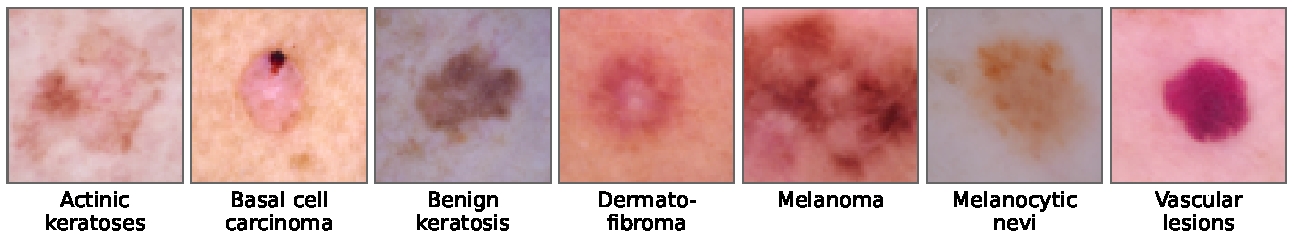
\includegraphics[width=0.7\textwidth]{F_dataset_classes.pdf}
\caption{DermaMNIST class distribution. Mel-nevi dominates at $66.9\,\%$ of
the training set; dermato ($1.1\,\%$), vascular ($1.4\,\%$), and melanoma
(${\approx}11\,\%$) define the rare-class set used throughout the chapter.}
\label{fig:dataset-classes}
\end{figure}



%%%%%%%%%%%%%%%%%%%%%%%%%%%%%%%%%%%%%%%%%%%%%%%%%%%%%%%%%%%%%%%%%%%%%%%%%%%%%%%
%% sec 5.2 -- Statistical heterogeneity alone gives limited optimiser separation
%%%%%%%%%%%%%%%%%%%%%%%%%%%%%%%%%%%%%%%%%%%%%%%%%%%%%%%%%%%%%%%%%%%%%%%%%%%%%%%

% =============================================================================
% Results sec 5.2 -- Statistical heterogeneity alone gives limited separation
% Compressed version. All numerics verified against VERIFICATION_SHEET.txt.
% Target ~500 words.
% =============================================================================

\section{Statistical heterogeneity alone gives limited optimiser separation}
\label{sec:statistical-heterogeneity}

Under an IID partition (Flower, $n=10$ paired seeds), FedAvg and FedProx
differ by $\Delta = -0.007$ macro-F1 (FA $0.585$, FP $0.578$, FN $0.577$) ---
within seed noise. We treat this as a negative control: statistical
heterogeneity is a necessary condition for any FedAvg--FedProx gap on this
benchmark.

On the engineered balanced-paired seven-client partition we report three
estimates ($n=10$ paired seeds each): Flower paired $\Delta = +0.007$ (7/10
paired wins, full \texttt{git\_commit} and \texttt{client\_update\_norms}
provenance), Flower $\mu$-sweep peak at $\mu = 0.01$ $\Delta = +0.013$ (full
provenance, $\mu$ characterisation in \S\,\ref{sec:mu-sensitivity}), and
pure-PyTorch reference $\Delta = +0.027$ (9/10 wins, no \texttt{git\_commit},
no companion update-norm logs). All three measure the same partition through
slightly different code paths; they agree on sign and bracket the magnitude
at $0.01$--$0.03$. The Flower paired $\Delta = +0.007$ is the central
headline; the pure-PyTorch number is cross-runtime corroboration.

The pure-PyTorch $+0.027$ is concentrated in two classes: melanoma
contributes $+0.114$ per-class F1 (61\,\% share of the macro-F1 advantage)
and actinic keratoses $+0.067$ (36\,\%); the other five classes contribute
the residual 3\,\% (all $|\Delta| \leq 0.013$), and mel-nevi is invariant at
$+0.002$. Figure~\ref{fig:engineered-per-class} renders the per-class
validation trajectories under the engineered partition ($n=10$ paired
seeds, $\pm 1$ SEM bands): the melanoma and actinic panels show non-
overlapping FedAvg vs FedProx bands by mid-training, while the other five
classes (including mel-nevi) overlap throughout 150 rounds. The gain
reflects rebalancing of two minority classes, not a uniform optimiser
improvement.

Three other partitions replicate the small-magnitude finding: Dirichlet
$\alpha = 0.1$ $\Delta = +0.008$ ($n=10$), specialist 1-of-7 $\Delta = +0.008$
($n=10$), multi-seed node-pinned L4 $\Delta = +0.005$ ($n=3$; per-seed
$\{+0.013, +0.019, -0.016\}$). The single-seed heterogeneity-ladder pilot
at L4 gives $\Delta = -0.030$, but its $-0.030$ deficit is driven entirely
by vascular F1 dropping by $-0.220$ (FA $0.702$ $\rightarrow$ FP $0.482$);
all six other classes are within $|\Delta| \leq 0.034$. The aggregate is one
rare-class outcome on one seed, and the $n=3$ node-pinned promotion
($\Delta = +0.005$) averages it out. All Dirichlet aggregates above use
regenerated raw-JSON summaries; the previously-committed analysis CSVs were
stale and showed a spurious seed-8675309 catastrophic FedProx failure that
the regenerated data do not support.

On the engineered partition, FedProx reduces test-macro-F1 SD from $0.025$
to $0.014$ ($-45\,\%$), reaches validation macro-F1 $= 0.40$ in $9.8$ vs
$12.7$ rounds ($1.3\times$ speed-up), and shows a paired mid-training peak
$\Delta = +0.094$ at round 50 that closes to $+0.007$ by round 150. These
trajectory characteristics are documented for the engineered partition only.

Statistical heterogeneity alone produces small, runtime-sensitive separation
(Table~\ref{tab:stat-het-headline}, Figure~\ref{fig:stat-het-forest}). The
next question is whether the proximal coefficient $\mu$ itself explains when
FedProx helps.


% =============================================================================
% Table 5.2 -- statistical heterogeneity and runtime sensitivity
% =============================================================================

\begin{table}[H]
\centering
\caption{Statistical heterogeneity and runtime sensitivity. Six cells:
IID, the engineered partition through two runtimes plus the $\mu$-peak,
Dirichlet $\alpha=0.1$, specialist 1-of-7, and the multi-seed node-pinned
L4 control. Dirichlet, specialist, and IID values from regenerated raw-JSON
aggregates.}
\label{tab:stat-het-headline}
\resizebox{\textwidth}{!}{%
\begin{tabular}{lccccccl}
\hline
Setting              & Runtime       & Clients & $n$ & FedAvg              & FedProx             & $\Delta$ & Note \\
\hline
IID                  & Flower        & 7       & 10  & $0.585 \pm 0.020$   & $0.578 \pm 0.020$   & $-0.007$ & negative control \\
Engineered (pure)    & pure-PyTorch  & 7       & 10  & $0.481 \pm 0.025$   & $0.508 \pm 0.014$   & $+0.027$ & 9/10 wins; partial provenance \\
Engineered (Flower)  & Flower        & 7       & 10  & $0.496$             & $0.503$             & $+0.007$ & 7/10 wins; \textbf{central} \\
Dirichlet $\alpha=0.1$ & Flower      & 7       & 10  & $0.480 \pm 0.036$   & $0.488 \pm 0.034$   & $+0.008$ & regenerated raw-JSON \\
Specialist 1-of-7    & Flower        & 7       & 10  & $0.437 \pm 0.024$   & $0.445 \pm 0.017$   & $+0.008$ & --- \\
Node-pinned L4       & Flower        & 2       & 3   & $0.492 \pm 0.019$   & $0.497 \pm 0.022$   & $+0.005$ & multi-seed L4 control \\
\hline
\end{tabular}%
}
\end{table}


% =============================================================================
% Figure 5.2(a) -- statistical heterogeneity forest plot
% =============================================================================

\begin{figure}[H]
\centering
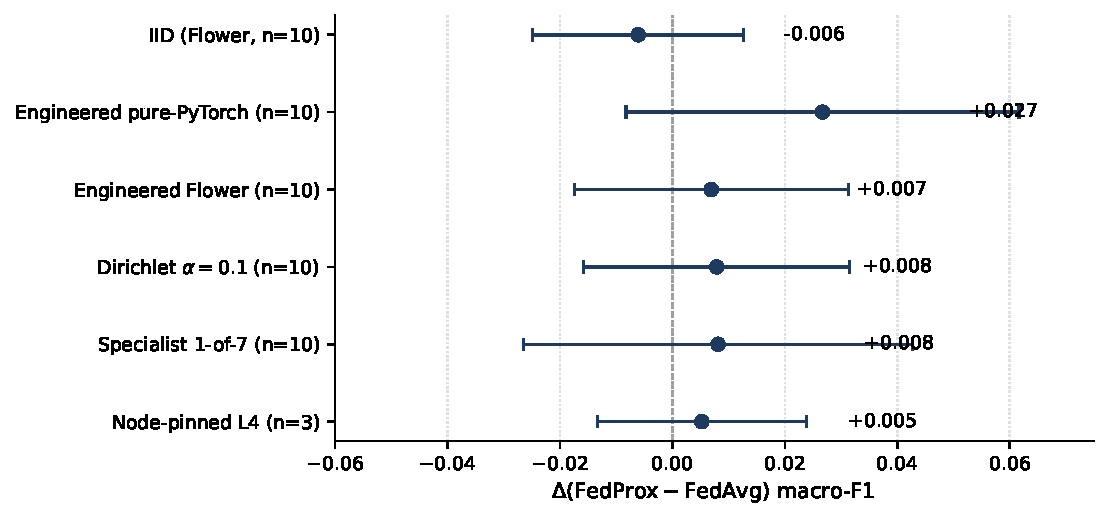
\includegraphics[width=0.85\textwidth]{F_statistical_heterogeneity_forest.pdf}
\caption{Forest plot of $\Delta(\textrm{FedProx} - \textrm{FedAvg})$ macro-F1
across the six settings in Table~\ref{tab:stat-het-headline}. Whiskers show
$\pm 1$ sample SD across paired seeds; dashed line at $\Delta = 0$ marks no
separation. The IID negative control sits at the left; the five partitioned
settings cluster between $+0.005$ and $+0.027$.}
\label{fig:stat-het-forest}
\end{figure}


% =============================================================================
% Figure 5.2(b) -- engineered partition per-class trajectories
% =============================================================================

\begin{figure}[H]
\centering

\includegraphics[width=\textwidth]{F_engineered_per_class.pdf}
\caption{Per-class validation F1 trajectories on the engineered partition,
$n = 10$ paired seeds (FedAvg vs FedProx, mean $\pm 1$ SEM bands).
Two-by-four grid (seven classes plus legend). Melanoma and actinic-keratoses
panels show non-overlapping FedAvg/FedProx bands by mid-training --- the
two classes that carry the pure-PyTorch $+0.027$ macro-F1 advantage
($+0.114$ and $+0.067$ per-class F1, $61\,\%$ and $36\,\%$ of the share
respectively). The other five classes show overlapping bands throughout
150 rounds, including the dominant mel-nevi panel which is invariant near
its prevalence saturation.}
\label{fig:engineered-per-class}
\end{figure}



%%%%%%%%%%%%%%%%%%%%%%%%%%%%%%%%%%%%%%%%%%%%%%%%%%%%%%%%%%%%%%%%%%%%%%%%%%%%%%%
%% sec 5.3 -- mu sensitivity: the proximal term helps only in a narrow range
%%%%%%%%%%%%%%%%%%%%%%%%%%%%%%%%%%%%%%%%%%%%%%%%%%%%%%%%%%%%%%%%%%%%%%%%%%%%%%%

% =============================================================================
% Results sec 5.3 -- mu sensitivity
% Compressed version. Target ~300 words.
% =============================================================================

\section{$\mu$ sensitivity: the proximal term helps only in a narrow range}
\label{sec:mu-sensitivity}

A five-cell sweep of $\mu \in \{0.001, 0.01, 0.1, 1.0\}$ against the FedAvg
baseline ($\mu = 0$) on the engineered partition ($n=10$ paired seeds per
cell) traces a clear inverted-$U$ (Table~\ref{tab:mu-sweep},
Figure~\ref{fig:mu-inverted-u}): peak near $\mu = 0.01$, dropping below
baseline by $\mu = 0.1$ and catastrophic at $\mu = 1.0$.

FedAvg gives $0.493 \pm 0.020$. FedProx at $\mu = 0.001$ reaches
$0.504 \pm 0.021$ ($\Delta = +0.011$, 6/10 paired wins); at $\mu = 0.01$ it
peaks at $0.506 \pm 0.017$ ($\Delta = +0.013$, 6/10 wins) --- numerically
indistinguishable from the $\mu = 0.001$ cell. At $\mu = 0.1$ the mean falls
to $0.479 \pm 0.017$ ($\Delta = -0.014$, 2/10 wins); at $\mu = 1.0$ it
collapses to $0.419 \pm 0.013$ ($\Delta = -0.074$, 0/10 wins --- every seed
loses). The $0.09$ macro-F1 spread between best and worst $\mu$ is an order
of magnitude larger than any partition-level $\Delta$ in
\S\,\ref{sec:statistical-heterogeneity}.

The $\mu$-sweep peak $\Delta = +0.013$ exceeds the
\S\,\ref{sec:statistical-heterogeneity} Flower paired $\Delta = +0.007$
because the sweep selects best-of-five on the same seeds; the two estimates
bracket the same small effect at $+0.005$ to $+0.015$.

The practical region of useful $\mu$ on this benchmark is a single decade
around $0.01$. The expectation that larger $\mu$ should be preferred under
stronger statistical heterogeneity is not supported here --- a benchmark
observation, not a refutation of the underlying analysis.

Table~\ref{tab:mu-per-class} breaks down the $\mu = 1.0$ catastrophic cell
per class. The deficit is concentrated in the rare and minority classes
(dermato $-0.101$, vascular $-0.113$, actinic $-0.124$) while the dominant
mel-nevi is essentially invariant ($-0.017$). The same rare-class
sensitivity that drives the catastrophic large-$\mu$ regime is the
clinical failure mode characterised in
\S\,\ref{sec:rare-class-collapse}; large-$\mu$ FedProx fails in the same
shape as the dropped-stragglers and asymmetric-LR cells, only via a
different mechanism (over-regularisation rather than under-aggregation).
Because $\mu$ alone is sensitive and at larger values harmful, the much
larger FedProx gains under straggler protocols
(\S\,\ref{sec:li-straggler}) cannot be attributed to the proximal
coefficient itself.


% =============================================================================
% Table 5.3 -- mu-sensitivity sweep
% =============================================================================

\begin{table}[H]
\centering
\caption{$\mu$ sensitivity on the engineered partition, $n=10$ paired
seeds per cell. ``Wins'' is paired comparisons where FedProx exceeds
FedAvg on the matched seed.}
\label{tab:mu-sweep}
\begin{tabular}{ccccl}
\hline
$\mu$    & macro-F1 (mean $\pm$ SD) & $\Delta$ vs FedAvg & Wins / 10 & Interpretation \\
\hline
$0$      & $0.493 \pm 0.020$        & ---               & ---       & FedAvg baseline                \\
$0.001$  & $0.504 \pm 0.021$        & $+0.011$          & 6         & near peak                      \\
$0.01$   & $\mathbf{0.506 \pm 0.017}$ & $\mathbf{+0.013}$ & 6       & \textbf{peak}                  \\
$0.1$    & $0.479 \pm 0.017$        & $-0.014$          & 2         & below baseline                 \\
$1.0$    & $0.419 \pm 0.013$        & $-0.074$          & 0         & catastrophic                   \\
\hline
\end{tabular}
\end{table}


% =============================================================================
% Figure 5.3 -- mu-sensitivity curve
% =============================================================================

\begin{figure}[H]
\centering
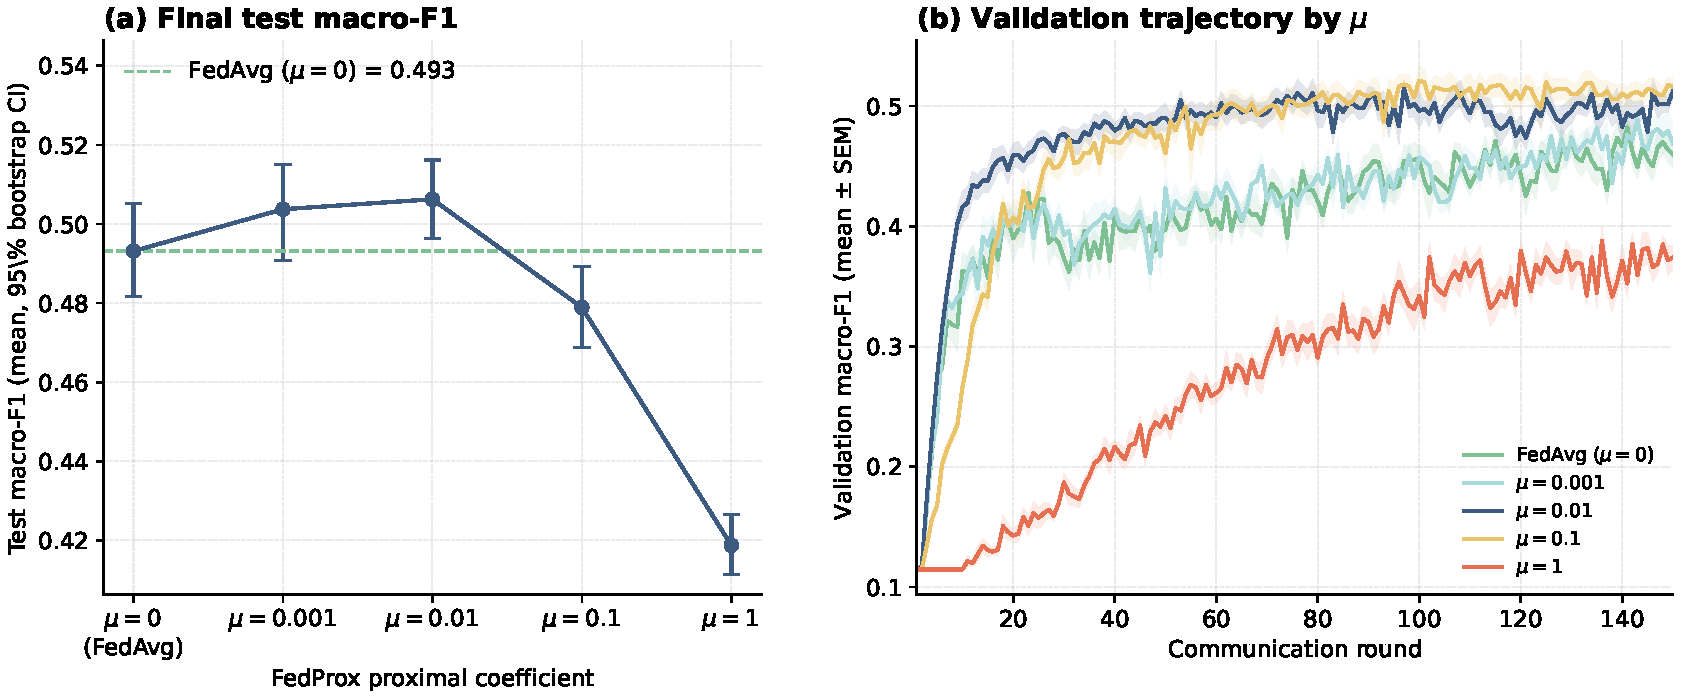
\includegraphics[width=0.85\textwidth]{F_mu_sensitivity_outcome_and_convergence.pdf}
\caption{Inverted-$U$ $\mu$ sensitivity curve on the engineered partition
($n=10$ per cell). $x$-axis: $\mu$ on $\log_{10}$ scale across
$\{0.001, 0.01, 0.1, 1.0\}$, FedAvg baseline as dashed reference line at
$0.493$. $y$-axis: test macro-F1 with $\pm 1$ SD whiskers.}
\label{fig:mu-inverted-u}
\end{figure}


% =============================================================================
% Table 5.3b -- per-class mu sensitivity (engineered partition)
% =============================================================================

\begin{table}[H]
\centering
\small
\caption{Per-class validation F1 mean across the $\mu$ sweep on the
engineered partition, $n = 10$ paired seeds per cell. SDs across seeds
range $0.003$ (mel-nevi) to $0.113$ (rare classes). ``$\Delta$ at $\mu=1.0$''
is the absolute per-class F1 deficit at the catastrophic cell relative to
the FedAvg baseline ($\mu = 0$). The deficit concentrates in rare and
minority classes; the dominant mel-nevi class is essentially invariant.
Source: \texttt{mu\_sensitivity\_flower/}.}
\label{tab:mu-per-class}
\resizebox{\textwidth}{!}{%
\begin{tabular}{lcccccc}
\hline
Class       & $\mu = 0$ & $\mu = 0.001$ & $\mu = 0.01$ & $\mu = 0.1$ & $\mu = 1.0$ & $\Delta$ at $\mu = 1.0$ \\
\hline
actinic     & $0.475$   & $0.470$       & $0.489$      & $0.434$     & $0.351$     & $-0.124$ \\
basal       & $0.497$   & $0.513$       & $0.497$      & $0.405$     & $0.438$     & $-0.060$ \\
b-kerat     & $0.405$   & $0.400$       & $0.423$      & $0.416$     & $0.328$     & $-0.077$ \\
dermato     & $0.259$   & $0.287$       & $0.283$      & $0.279$     & $0.158$     & $\mathbf{-0.101}$ \\
melanoma    & $0.244$   & $0.258$       & $0.304$      & $0.287$     & $0.216$     & $-0.028$ \\
mel-nevi    & $0.884$   & $0.885$       & $0.886$      & $0.886$     & $0.867$     & $-0.017$ \\
vascular    & $0.687$   & $0.713$       & $0.661$      & $0.646$     & $0.574$     & $\mathbf{-0.113}$ \\
\hline
\end{tabular}%
}
\end{table}



%%%%%%%%%%%%%%%%%%%%%%%%%%%%%%%%%%%%%%%%%%%%%%%%%%%%%%%%%%%%%%%%%%%%%%%%%%%%%%%
%% sec 5.4 -- Li-style straggler asymmetry (CENTREPIECE)
%%%%%%%%%%%%%%%%%%%%%%%%%%%%%%%%%%%%%%%%%%%%%%%%%%%%%%%%%%%%%%%%%%%%%%%%%%%%%%%

% =============================================================================
% Results sec 5.4 -- Centrepiece
% Compressed version. Target ~720 words (centrepiece stays substantive).
% =============================================================================

\section{Under Li-style straggler asymmetry, FedProx's advantage is mediated
mainly by $\gamma$-inexact partial-update handling}
\label{sec:li-straggler}

Before decomposing the mechanism, we first tested whether stragglers by
themselves were enough to create a FedProx advantage. They were not. In a
7-client IID random-straggler control, all clients had similar label
distributions, while a random subset of clients completed reduced local
training in each round. In that setting, FedProx was slightly worse than
FedAvg ($\Delta = -0.013$ macro-F1, $n = 10$). We then kept the same
7-client random-straggler protocol but replaced the IID data split with a
heterogeneous split, so that class information was no longer evenly shared
across clients. The sign reversed: FedProx exceeded FedAvg by $+0.017$
macro-F1 ($n = 10$). This first comparison is therefore a screening
result: random stragglers alone do not explain the effect; the advantage
appears only when slow or partially updated clients may also carry
non-redundant class information. The next experiment tests that mechanism
directly in a separate two-client L4 decomposition, where the rare-class
client is deliberately made the fixed straggler.

We next isolate the mechanism in a two-client L4 four-condition experiment,
with $n=3$ matched seeds (Table~\ref{tab:li-decomp-l4}). In this setting,
Client 1 contains the rare-class signal and is made the fixed straggler. The
four cells separate two effects that are otherwise bundled together in
FedProx-style straggler experiments: the proximal term and the decision to
accept or drop a straggler's partial update.

\begin{table}[H]
\centering
\caption{Li-style four-condition decomposition at L4 (two-client; $n=3$
matched seeds; mean $\pm$ sample SD across seeds).}
\label{tab:li-decomp-l4}
\small
\begin{tabular}{lcc}
\toprule
Condition                                       & Test macro-F1                & Rare-class F1 \\
\midrule
FedAvg, no straggler                            & $0.485 \pm 0.028$            & $0.316 \pm 0.060$ \\
FedAvg + drop                                   & $0.364 \pm 0.009$            & $0.000 \pm 0.000$ \\
FedProx + drop (control)                        & $0.368 \pm 0.005$            & $0.000 \pm 0.000$ \\
FedProx + $\gamma$-inexact                      & $\mathbf{0.479 \pm 0.010}$   & $\mathbf{0.291 \pm 0.018}$ \\
\bottomrule
\end{tabular}

\smallskip
\noindent\textit{Decomposition:} proximal-only $= 0.368 - 0.364 = +0.004$;
$\gamma$-inexact $= 0.479 - 0.368 = +0.111$; total $= +0.115$. Rare-F1 is
the mean over $\mathrm{RARE\_IDX} = \{\text{dermato}, \text{melanoma},
\text{vascular}\}$ and shows that the macro-F1 gap lives entirely in the
rare classes: both drop-handling cells flatline rare-F1 to exactly zero,
and only FedProx+$\gamma$-inexact rescues it.
\end{table}

The first two cells measure the cost of straggling under FedAvg. FedAvg with
no straggler reaches $0.485 \pm 0.028$ macro-F1. When the straggler's partial
update is dropped, performance falls to $0.364 \pm 0.009$, a drop of
$0.121$. This shows that the straggler is not just slow; in L4, dropping it
removes important class information.

The next two cells identify what recovers that loss. Adding the FedProx
proximal term while still dropping the straggler changes almost nothing:
FedProx+drop reaches $0.368 \pm 0.005$, only $+0.004$ above FedAvg+drop.
By contrast, FedProx+$\gamma$-inexact reaches $0.479 \pm 0.010$, a
$+0.111$ gain over FedProx+drop and almost a return to the no-straggler
baseline. Thus, within this design, the large FedProx straggler-regime
advantage is driven mainly by accepting the rare client's partial update,
not by the proximal regulariser alone.

Equivalently, the total gain from FedAvg+drop to FedProx+$\gamma$-inexact
is $+0.115$. Of this, only $+0.004$ comes from the proximal term under
matched drop-handling, while $+0.111$, or about $96\%$, comes from
accepting the partial update. Because the design does not include a
FedAvg+$\gamma$-inexact cell, this should be read as evidence for the
FedProx+$\gamma$-inexact protocol, not as proof that $\gamma$-inexact
acceptance is universally beneficial on its own.

Figure~\ref{fig:val-curves-extreme-gaps}~(A) shows the same result over
training. FedAvg+drop and FedProx+drop follow almost the same validation
trajectory for all 150 rounds, so the proximal term does not materially
change the convergence path when the rare client is still dropped.
FedProx+$\gamma$-inexact separates from both curves around round 30 and
stabilises near $0.48$, showing that the improvement comes from keeping the
straggler's partial contribution in aggregation.

\begin{figure}[H]
\centering
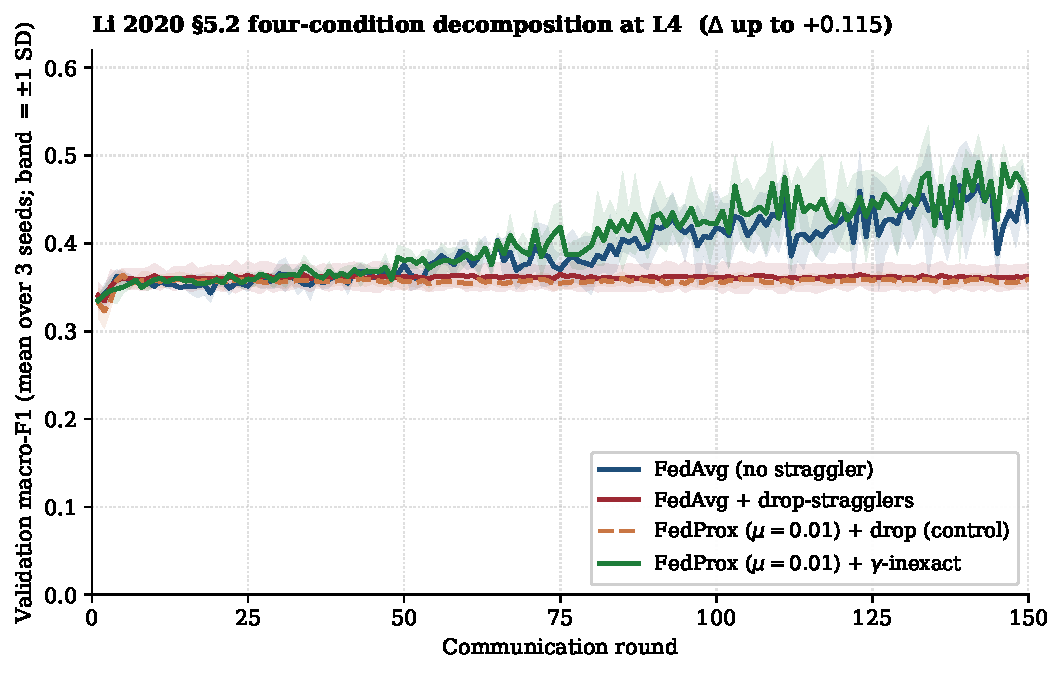
\includegraphics[width=\textwidth]{F_val_curves_l4_four_condition.pdf}
\caption{Li 2020 §5.2 four-condition decomposition at L4: validation
macro-F1 trajectories (mean over three seeds; shaded bands are $\pm 1$
sample SD). The FedAvg+drop and FedProx+drop trajectories overlap
throughout 150 rounds, isolating the proximal term as inactive under
matched drop-handling. Only FedProx+$\gamma$-inexact separates and
recovers towards the no-straggler baseline. The perfect-storm convergence
trajectories (random $90\%$ straggler regime) are reproduced in
Appendix~C.}
\label{fig:val-curves-extreme-gaps}
\end{figure}

The per-class trajectories in Figure~\ref{fig:l4-per-class-grid} show where
this aggregate gain comes from. The dominant mel-nevi class remains near
$0.89$ under all four conditions, so the improvement is not driven by the
majority class. The rare classes tell the opposite story: dermato, melanoma,
and vascular collapse under both drop-handling conditions, then recover most
clearly under FedProx+$\gamma$-inexact. The mechanism is therefore localised
to rare-class learning, not to a broad improvement across all classes.

\begin{figure}[H]
\centering
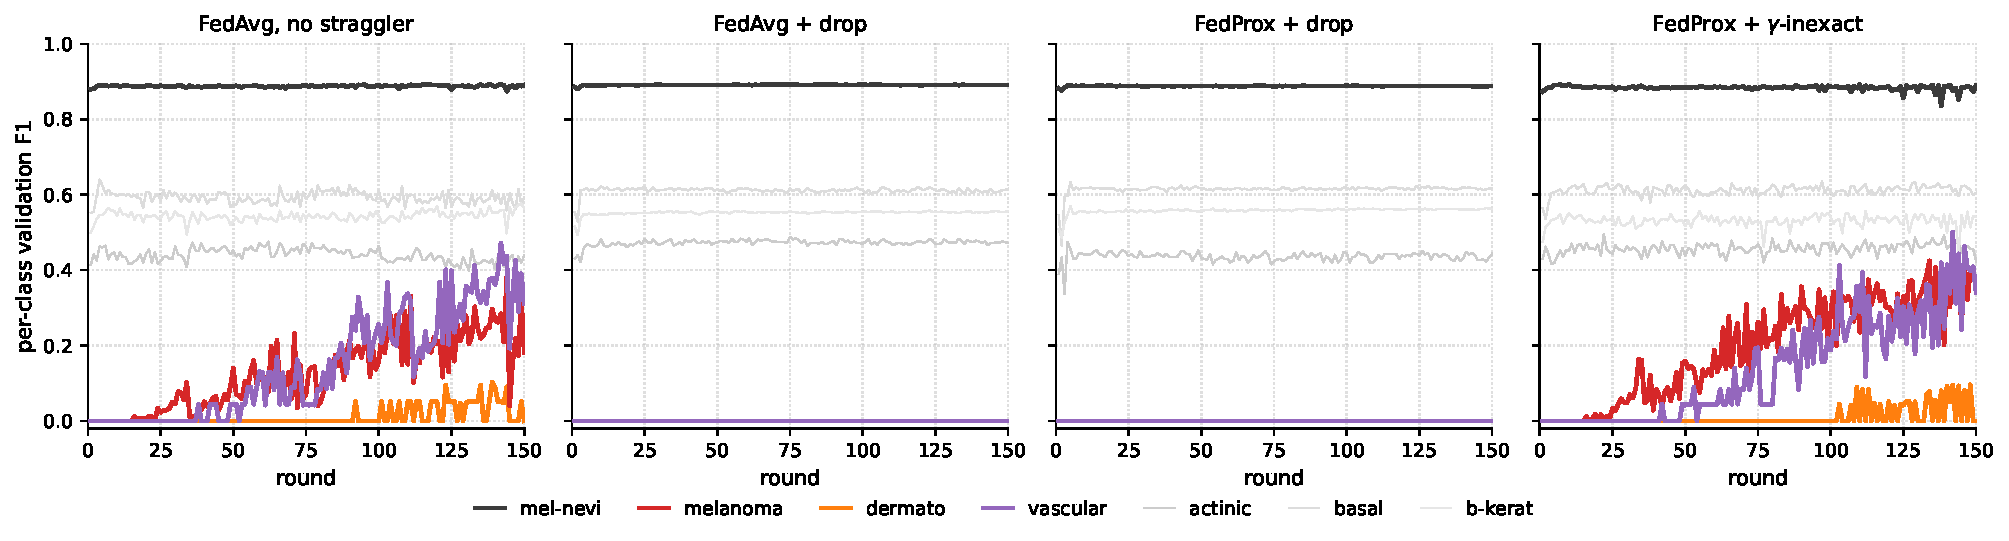
\includegraphics[width=\textwidth]{F_l4_four_condition_per_class_grid.pdf}
\caption{Per-class validation F1 trajectories under the four conditions of
the L4 decomposition (Table~\ref{tab:li-decomp-l4}); mean over three seeds.
The majority class (mel-nevi) stays near $0.89$ in every cell, so the
aggregate improvement is not driven by the dominant class. The three rare
classes (dermatofibroma, melanoma, vascular) collapse under both
drop-handling cells and recover most clearly under
FedProx+$\gamma$-inexact, identifying rare-class learning as the locus of
the mechanism.}
\label{fig:l4-per-class-grid}
\end{figure}

The perfect-storm experiment is a stress demonstration of the same ordering,
not a second causal decomposition. It keeps the L4 setting but makes
straggling more severe (random $90\%$ per-round straggler rate, batch size
$10$, no momentum) and compares FedAvg+drop with two FedProx+$\gamma$-inexact
arms. The contrast produces the \emph{largest FedProx--FedAvg macro-F1 gap
measured anywhere in this thesis}: $\Delta = +0.404$ (FedProx
$\mu = 0.01$ minus FedAvg+drop). FedAvg+drop flatlines at the round-1
validation value for every seed --- the best-val checkpoint is the untrained
random init for all three seeds, giving a mean test macro-F1 of
$0.087 \pm 0.049$. FedProx+$\gamma$-inexact recovers to $0.365 \pm 0.023$ at
$\mu = 1.0$ and to $0.491 \pm 0.003$ at $\mu = 0.01$.

\paragraph{Why is the gap so large?}
The mechanism is the same information-flow asymmetry that the L4
decomposition isolated, but the perfect storm pushes it to its limit. At
each round the server samples participating clients independently with
$P(\text{straggle}) = 0.9$; when both clients straggle, FedAvg+drop has
nothing to aggregate and the global model is unchanged. In the L4
two-client setting, this means that the rare-class client (Client 1)
contributes a full update to roughly only one round in ten, and a partial
update never --- because partial updates are discarded. The global model
therefore moves almost exclusively along Client 0's gradient direction,
which is the dominant-class direction; rare-class logits decay and the
validation macro-F1 stops improving after the first round. Best-val
checkpointing then returns the untrained init, because no later round ever
beats it. FedProx+$\gamma$-inexact breaks this collapse by a single
structural change: stragglers contribute the partial work they did manage,
so Client 1's rare-class gradient enters aggregation in essentially every
round even when its local training was incomplete. The proximal term
$\tfrac{\mu}{2}\lVert w - w^t \rVert^2$ keeps those partial updates from
drifting too far from the previous round's anchor, which is why the smaller
$\mu = 0.01$ (looser anchoring, more learning signal per round) outperforms
$\mu = 1.0$ here. The $+0.404$ gap therefore measures the difference
between information loss (FedAvg+drop silently discarding the only client
that holds rare-class signal) and information rescue (FedProx+$\gamma$-inexact
preserving that signal under the same client schedule).

The perfect-storm result confirms that the L4 ordering survives a harsher
straggler regime, but it does not replace the four-condition decomposition
because several settings change at once (straggler rate, batch size,
momentum) and the FedAvg+drop arm collapses too completely for a clean
$\gamma$-inexact-vs-proximal split.

Finally, the L1 control tests whether partial-update acceptance helps simply
because it is a better generic straggler policy. It does not. L1 uses the
same two-client four-condition design, but the clients have identical label
proportions; the split changes quantity, not class information. In this
setting, all four cells are nearly flat (Table~\ref{tab:li-decomp-l1}):
FedAvg-no-straggler $0.601 \pm 0.010$, FedAvg+drop $0.599 \pm 0.006$,
FedProx+drop $0.593 \pm 0.022$, and FedProx+$\gamma$-inexact
$0.605 \pm 0.009$. Dropping the straggler costs almost nothing, and accepting
the partial update adds only $+0.012$, compared with $+0.111$ at L4.

\begin{table}[H]
\centering
\caption{L1 cross-partition control: same four-condition design as
Table~\ref{tab:li-decomp-l4} but on the L1 partition (quantity-only
heterogeneity, JS divergence $\approx 0$); $n=3$ matched seeds, mean
$\pm$ sample SD. The proximal-only and $\gamma$-inexact contributions both
collapse toward zero relative to L4, which is the cleanest negative
control for the rare-class-signal-rescue mechanism interpretation.}
\label{tab:li-decomp-l1}
\small
\begin{tabular}{lcc}
\toprule
Condition                                       & Test macro-F1        & Rare-class F1 \\
\midrule
FedAvg, no straggler                            & $0.601 \pm 0.010$    & $0.530 \pm 0.008$ \\
FedAvg + drop                                   & $0.599 \pm 0.006$    & $0.539 \pm 0.012$ \\
FedProx + drop (control)                        & $0.593 \pm 0.022$    & $0.537 \pm 0.039$ \\
FedProx + $\gamma$-inexact                      & $0.605 \pm 0.009$    & $0.556 \pm 0.014$ \\
\bottomrule
\end{tabular}

\smallskip
\noindent\textit{Decomposition (vs L4 in parentheses):}
proximal-only $= 0.593 - 0.599 = -0.006$ (L4: $+0.004$);
$\gamma$-inexact $= 0.605 - 0.593 = +0.012$ (L4: $+0.111$);
drop-cost $= 0.601 - 0.599 = +0.002$ (L4: $+0.121$). The $\gamma$-inexact
contribution shrinks by an order of magnitude when the dropped client
carries no class signal the other client lacks. The rare-F1 column makes
this concrete: at L1 every cell sits in $0.53$--$0.56$ (a $\pm 0.026$
band), while at L4 the two drop cells crash to exactly zero and only
$\gamma$-inexact recovers rare-F1 to $0.29$. There is nothing to rescue
when the dropped client carries no unique rare-class signal.
\end{table}

The L4/L1 contrast is therefore the key mechanism evidence. At L4, the
dropped client carries class information the other client does not have, so
accepting its partial update rescues rare-class learning. At L1, the dropped
client carries no unique class signal, so there is little to rescue. The
straggler mechanism is not generic drift control; it matters when system
heterogeneity suppresses statistically unique rare-class information.

The straggler experiments isolate one axis of system asymmetry.
Section~\ref{sec:lr-asymmetry} asks whether persistent learning-rate
imbalance --- a different axis --- changes the optimiser ranking.



%%%%%%%%%%%%%%%%%%%%%%%%%%%%%%%%%%%%%%%%%%%%%%%%%%%%%%%%%%%%%%%%%%%%%%%%%%%%%%%
%% sec 5.5 -- Learning-rate asymmetry reveals FedNova regime-dependence
%%%%%%%%%%%%%%%%%%%%%%%%%%%%%%%%%%%%%%%%%%%%%%%%%%%%%%%%%%%%%%%%%%%%%%%%%%%%%%%

% =============================================================================
% Results sec 5.5 -- Learning-rate asymmetry, FedNova regime-dependence
% =============================================================================

\section{Learning-rate asymmetry reveals FedNova regime-dependence}
\label{sec:lr-asymmetry}

This experiment tests a different form of system heterogeneity from
\S\,\ref{sec:li-straggler}. There, the rare-class client was slow and its
partial update could be dropped. Here, the rare-class client is not dropped:
it still participates in every round, but its learning rate is made smaller.
The question is whether an optimiser can preserve rare-class learning when
the rare client's update becomes progressively weaker.

The experiment is run on L4. Client 0 is the dominant client and keeps
$\textrm{lr}=0.01$ throughout. Client 1 holds the rare classes and is assigned
one of six smaller learning rates, producing asymmetry ratios from 1:1 to
50:1. Each ratio is tested with FedAvg, FedProx, and FedNova using $n=3$
matched seeds per cell, giving $54$ runs in total. Test macro-F1 across the
six-ratio envelope is reported below.

\begin{center}
\resizebox{\textwidth}{!}{%
\begin{tabular}{c|cc|ccc|cc}
\hline
Ratio & Client 0 lr & Client 1 lr & FedAvg & FedProx & FedNova & FN$-$FA & FN$-$FP \\
\hline
 1:1  & $0.01$ & $0.01$    & $0.457$ & $0.491$ & $\mathbf{0.509}$ & $+0.052$ & $+0.018$ \\
 2:1  & $0.01$ & $0.005$   & $0.425$ & $0.462$ & $\mathbf{0.526}$ & $+0.101$ & $+0.064$ \\
 5:1  & $0.01$ & $0.002$   & $0.375$ & $0.392$ & $\mathbf{0.504}$ & $+0.129$ & $+0.112$ \\
10:1  & $0.01$ & $0.001$   & $0.369$ & $0.369$ & $\mathbf{0.501}$ & $+0.132$ & $+0.132$ \\
20:1  & $0.01$ & $0.0005$  & $0.367$ & $0.372$ & $\mathbf{0.486}$ & $+0.119$ & $+0.114$ \\
50:1  & $0.01$ & $0.0002$  & $0.367$ & $0.367$ & $\mathbf{0.498}$ & $\mathbf{+0.131}$ & $\mathbf{+0.131}$ \\
\hline
\end{tabular}%
}
\end{center}

The pattern is clear. FedAvg and FedProx both degrade as soon as Client 1's
learning rate is reduced. Between the symmetric 1:1 setting and the 5:1
setting, FedAvg falls from $0.457$ to $0.375$, while FedProx falls from
$0.491$ to $0.392$. After that, both methods plateau near $0.367$ macro-F1.
This plateau is the rare-class floor: the model still learns parts of the
dominant-client distribution, but rare-class learning has largely collapsed.

FedNova behaves differently. Its macro-F1 remains between $0.486$ and
$0.526$ across the full 1:1--50:1 envelope. Even at 50:1, where Client 1's
learning rate is fifty times smaller than Client 0's, FedNova reaches
$0.498$ macro-F1, compared with $0.367$ for both FedAvg and FedProx. The
FedNova--FedAvg gap at 50:1 is therefore $+0.131$ macro-F1.

The rare-class F1 confirms that this is not just a macro-F1 artefact. At
10:1, rare-class F1 is already almost zero for FedAvg and FedProx
(FA $0.016$, FP $0.010$), and by 50:1 it is approximately zero. FedNova keeps
rare-class F1 much higher throughout the envelope, with $0.366$ at 10:1 and
$0.353$ at 50:1. Figure~\ref{fig:lr-asymmetry-envelope} shows both views:
overall macro-F1 and rare-class F1.

\begin{figure}[H]
\centering
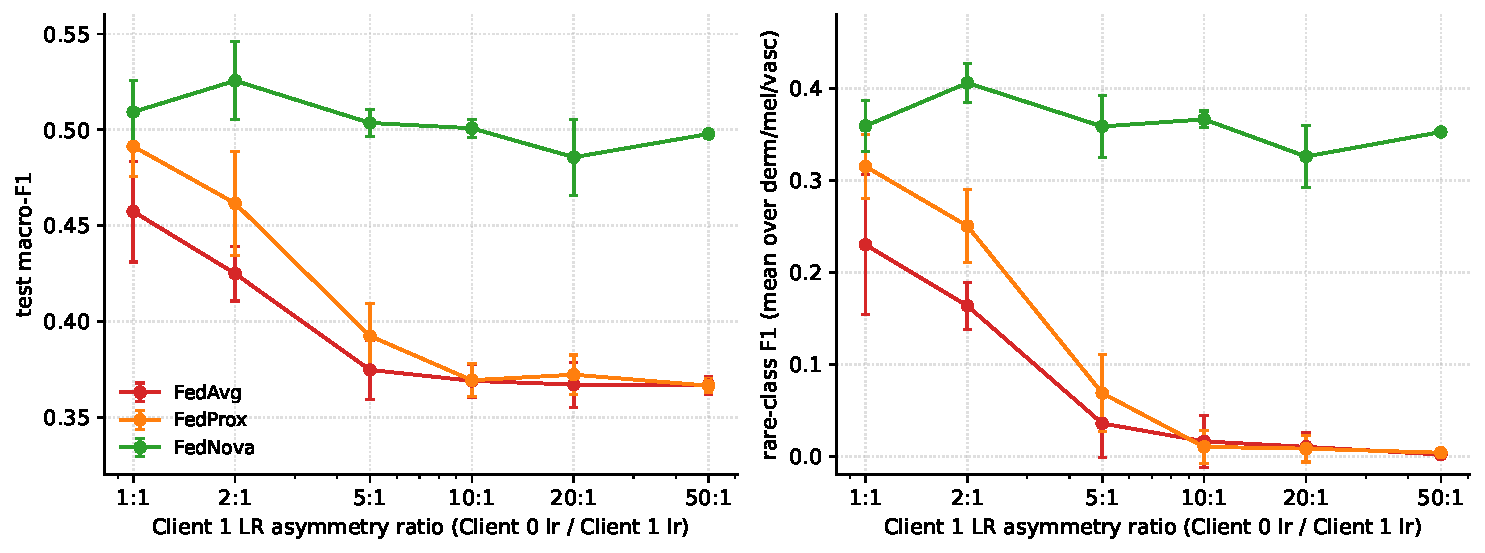
\includegraphics[width=\textwidth]{F_asymmetric_lr_L4.pdf}
\caption{Learning-rate asymmetry envelope at L4, $n=3$ per cell. Two
panels: test macro-F1 and rare-class F1 (mean over dermato, melanoma,
vascular) vs the Client 1 LR ratio on a $\log_{10}$ axis from 1:1 to 50:1.
FedAvg and FedProx plateau at the rare-class floor; FedNova stays flat
across the envelope.}
\label{fig:lr-asymmetry-envelope}
\end{figure}

The 5:1 cell is also where the chapter's metric choice earns its keep. Mean
test accuracy across the three matched seeds is $0.753$ for FedAvg and
$0.726$ for FedNova: ranking by raw accuracy would prefer FedAvg, even
though its macro-F1 ($0.375$) and rare-class F1 ($\approx 0.02$) make it
clear that FedAvg has lost the rare-class signal almost entirely while
FedNova has not (macro-F1 $0.504$, rare-F1 $\approx 0.37$). The accuracy
gap is small precisely because both models still get mel-nevi
($66.9\,\%$ of the test set) right; macro-F1 separates them because it
weights all seven classes equally. This is the operational reason \S\,5.1
ranks optimisers by macro-F1 and never by accuracy.

A simple interpretation is that FedAvg and FedProx allow the rare client's
update to become too small. When Client 1's learning rate is reduced, its
local model moves less during training, so the update it sends back to the
server carries weaker rare-class information. FedAvg does not correct this,
and the FedProx proximal term does not restore a rare-client update that has
already become too small. FedNova, by contrast, normalises client updates by
effective local work, which helps preserve Client 1's contribution in this
deterministic asymmetry setting.

The update-norm logs support this reading. At the 5:1 cell, Client 1's mean
update size relative to its own 1:1 update is $0.47$ for FedAvg and $0.50$
for FedProx, but $0.91$ for FedNova. In other words, FedAvg and FedProx let
the rare-client update shrink by roughly half, while FedNova keeps it much
closer to its original size. This is mechanism-consistent evidence, not a
causal proof, but it matches the rare-class F1 pattern.

FedNova's success here is not universal. The same method fails under
random-$\tau$ straggler heterogeneity. In that setting, the amount of local
work changes randomly from round to round. FedNova obtains only
$0.237 \pm 0.094$ macro-F1, far below the matching FedAvg and FedProx cells
(FA $0.493$, FP $0.510$ from \S\,\ref{sec:li-straggler}). Three of ten seeds
collapse to macro-F1 $=0.114$, the majority-class-only baseline obtained by
predicting mel-nevi for every test image.

This contrast is the main point of the section. FedNova is robust when the
asymmetry is stable and deterministic: the rare client is consistently
weakened, and normalisation can compensate. It is brittle when the amount of
local work is random and noisy: normalisation can then amplify unstable
partial updates instead of correcting them. FedNova is therefore
regime-dependent, not universally superior.

\begin{center}
\begin{tabular}{p{0.22\linewidth}p{0.32\linewidth}p{0.38\linewidth}}
\hline
FedNova regime & Result & Interpretation \\
\hline
Persistent LR asymmetry & macro-F1 holds $0.49$--$0.53$ across 1:1--50:1 & $\tau$-normalisation preserves smaller client's contribution \\
Random-$\tau$ stragglers & macro-F1 $= 0.237 \pm 0.094$; 3/10 majority collapse & $\tau$-normalisation amplifies noisy partial updates (outside Wang 2020) \\
\hline
\end{tabular}
\end{center}

Figure~\ref{fig:heterogeneity-escalation} places the large FedAvg--FedProx
gaps from the previous section on one axis. The progression from IID to
symmetric L4 to Li-style straggler asymmetry and then to perfect-storm shows
that optimiser gaps become large only in specific stress regimes. Together
with the FedNova result above, this reinforces the chapter's central point:
the optimiser ranking depends on the heterogeneity regime, not on the
optimiser name alone.

\begin{figure}[H]
\centering
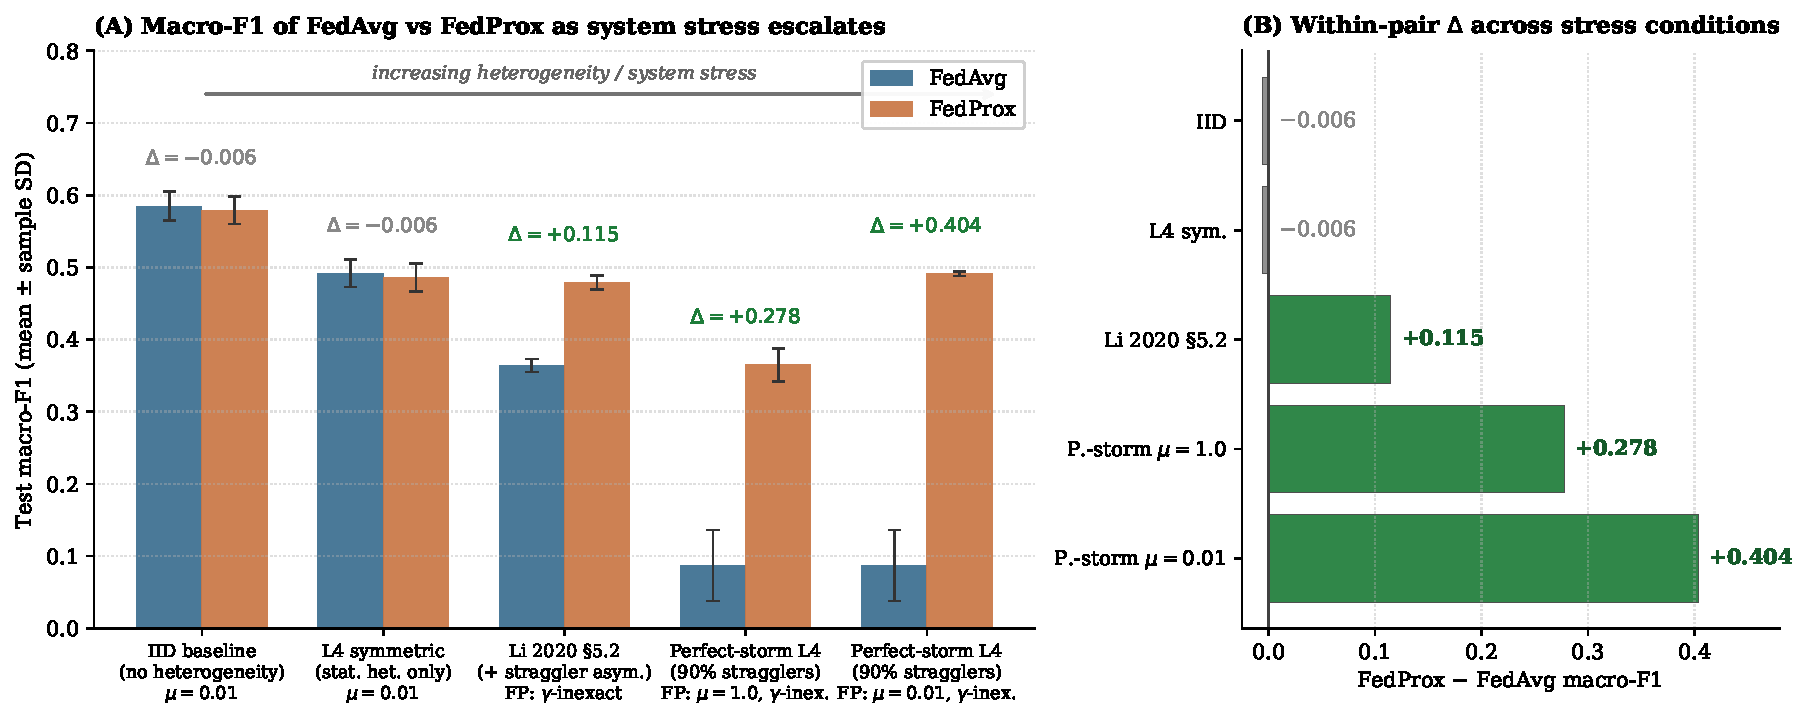
\includegraphics[width=0.85\textwidth]{F_heterogeneity_escalation.pdf}
\caption{Heterogeneity-escalation synthesis. Within-pair
$\Delta(\textrm{FedProx} - \textrm{FedAvg})$ macro-F1 across five regime
cells of increasing severity: IID Flower negative control ($-0.007$),
symmetric L4 multi-seed node-pinned ($+0.005$), Li 2020 four-condition
contrast (FA+drop vs FP+$\gamma$-inex, $+0.115$), perfect-storm
$\mu = 1.0$ ($+0.278$), perfect-storm $\mu = 0.01$ ($+0.404$). The first
two cells sit inside seed noise; the last three are large,
mechanism-isolable, and regime-driven.}
\label{fig:heterogeneity-escalation}
\end{figure}

The weak protocols fail in a clinically specific way: they lose rare-class
sensitivity. The next section shows that this failure usually appears as
rare-class images being routed into the dominant mel-nevi class.



%%%%%%%%%%%%%%%%%%%%%%%%%%%%%%%%%%%%%%%%%%%%%%%%%%%%%%%%%%%%%%%%%%%%%%%%%%%%%%%
%% sec 5.6 -- Rare-class collapse into mel-nevi
%%%%%%%%%%%%%%%%%%%%%%%%%%%%%%%%%%%%%%%%%%%%%%%%%%%%%%%%%%%%%%%%%%%%%%%%%%%%%%%

% =============================================================================
% Results sec 5.6 -- Rare-class collapse + loss-side correction
% Compressed version. Target ~470 words.
% =============================================================================

\section{Rare-class collapse into mel-nevi, and why FedProx is not simply
an imbalance corrector}
\label{sec:rare-class-collapse}


\subsection*{\S\,5.6.1 Per-class collapse}

The low-macro-F1 cells in \S\S\,\ref{sec:li-straggler}--\ref{sec:lr-asymmetry}
fail the same way: rare-class images are routed to mel-nevi
(Figure~\ref{fig:cross-experiment-per-class}). Mean rare-to-mel-nevi
misrouting (over dermato, melanoma, vascular) ranges from $24\,\%$ in the
best protocol (perfect-storm FP $\mu = 0.01$, $n=3$) to $67\,\%$ in the
worst (perfect-storm FA+drop, $n=3$), and $28\,\%$ even under the IID
Flower negative control ($n=10$) --- a class-imbalance saturation that the
FL protocol preserves or amplifies but does not itself create.

The D1 5:1 cell isolates the optimiser dimension: melanoma per-class F1 is
$1.20\,\%$ for FedAvg, $6.13\,\%$ for FedProx, $46.34\,\%$ for FedNova
($n=3$ each) --- same disease, three detection regimes spanning two orders
of magnitude. Macro-F1 is structurally sensitive: each class enters with
weight $1/7$, so a single class dropping from per-class F1 $\approx 0.4$ to
$0.0$ moves macro by $\approx 0.057$, the order of the entire engineered
$\Delta$ in \S\,\ref{sec:statistical-heterogeneity}. The same
rare-class-concentration pattern reappears in the
\S\,\ref{sec:mu-sensitivity} $\mu = 1.0$ catastrophic cell
(Table~\ref{tab:mu-per-class}, where dermato loses $-0.101$, vascular
$-0.113$, and mel-nevi is invariant), so across three different mechanisms
--- aggregation dropout, learning-rate asymmetry, and over-regularisation
--- failure expresses itself in the same rare-class shape.

\begin{center}
\small
\begin{tabular}{p{0.16\linewidth} p{0.14\linewidth} c c c p{0.32\linewidth}}
\hline
Protocol                  & Algorithm & Rare-F1 & Melanoma F1 & Misrouting & Interpretation \\
\hline
Perfect-storm + drop      & FedAvg    & $0.000$ & $0.00\,\%$  & $67\,\%$   & Rare client dropped; flatline \\
Perfect-storm + $\gamma$  & FedProx ($\mu=0.01$) & $0.357$ & $38.27\,\%$ & $24\,\%$ & $\gamma$-inex preserves rare signal \\
D1 5:1 LR asymmetry       & FedAvg    & $0.036$ & $1.20\,\%$  & $51\,\%$   & Rare client under-weighted; gradual erosion \\
D1 5:1 LR asymmetry       & FedNova   & $0.359$ & $46.34\,\%$ & $26\,\%$   & $\tau$-normalisation preserves contribution \\
\hline
\end{tabular}
\end{center}

\noindent
These four cells span instant-collapse and gradual-erosion modes across
straggler and LR-asymmetry axes; the misrouting rate co-varies with rare-F1
across all four.


\subsection*{\S\,5.6.2 Collapse modes}

Two trajectories of the same failure mode. Perfect-storm FedAvg+drop's
validation trajectory flatlines at each seed's round-1 value for all 150
rounds (best-val checkpoint selected at round 1, untrained init beating
every trained checkpoint; across-seed mean test macro-F1 $= 0.087 \pm 0.049$):
the rare-class client is dropped every round, so its signal has no path
into the global parameters. D1 5:1 degrades gradually instead: the rare client's updates
are accepted but progressively under-weighted, macro-F1 drifts $0.457 \to
0.375$ with rare-F1 collapsing in lockstep. Instant collapse and gradual
erosion of the same rare-class-signal-suppression mechanism, distinguished
only by whether the rare-class updates are dropped wholesale or simply
under-weighted.


\subsection*{\S\,5.6.3 Loss-side imbalance correction: weighted CE and
focal loss}

To test whether the FedProx advantage might be class-imbalance correction
in disguise, we ran FedAvg and FedProx at L4 with three loss functions
($n=3$ per cell): plain cross-entropy, class-weighted CE with
inverse-frequency weights, and focal loss ($\gamma = 2$). Cells are test
macro-F1 $\pm$ SD with rare-class F1 in parentheses.

\begin{center}
\begin{tabular}{lccc}
\hline
Algorithm & CE & Weighted CE & Focal \\
\hline
FedAvg  & $0.477 \pm 0.002$ ($0.285$) & $\mathbf{0.505 \pm 0.023}$ ($\mathbf{0.367}$) & $0.467 \pm 0.002$ ($0.317$) \\
FedProx & $0.478 \pm 0.016$ ($0.291$) & $0.503 \pm 0.014$ ($0.346$)                   & $0.476 \pm 0.022$ ($0.304$) \\
\hline
\end{tabular}
\end{center}

Three observations. (i) Weighted CE is the strongest loss-side correction:
FedAvg+wCE $0.505$ marginally exceeds FedProx+CE $0.478$ in this L4
symmetric setting; the FedAvg-only CE-to-wCE intervention raises macro by
$+0.029$ and rare-F1 by $+0.082$. (ii) Focal helps rare-F1 ($+0.032$ on
FedAvg) but hurts macro ($-0.010$): focal trades macro for rare-recall,
while wCE wins on both at the tested $\gamma=2$ and inverse-frequency
weights. (iii) FedProx adds little on top of either: FP+wCE
$0.503 \pm 0.014$ sits inside FA+wCE's SD of $0.023$, and FP/FA differ by
$0.009$ at focal. FedProx is a drift/protocol intervention (per
\S\,\ref{sec:li-straggler}), not a substitute for direct loss-side
imbalance correction; the two axes can in principle be combined but are
tested only separately here ($n=3$, L4 symmetric only).

The \S\,\ref{sec:li-straggler} FedProx + $\gamma$-inexact result and this
\S\,5.6.3 weighted-CE result are not in tension: $\gamma$-inex restores
aggregation under straggler-induced signal loss, while weighted CE
re-weights rare classes during local training. They act at different
pipeline stages and address different failure modes (signal loss vs label
saturation); they could in principle be combined but are tested only
separately here.

The rare-class collapse documented here is clinically \emph{motivated},
not clinically \emph{validated}: DermaMNIST is a $28 \times 28$-pixel
benchmark and not a deployment artefact. The next section turns to the
per-round update-norm activity behind these per-class outcomes.


% =============================================================================
% Figure 5.7 -- cross-experiment per-class diagonal accuracy
% =============================================================================

\begin{figure}[H]
\centering
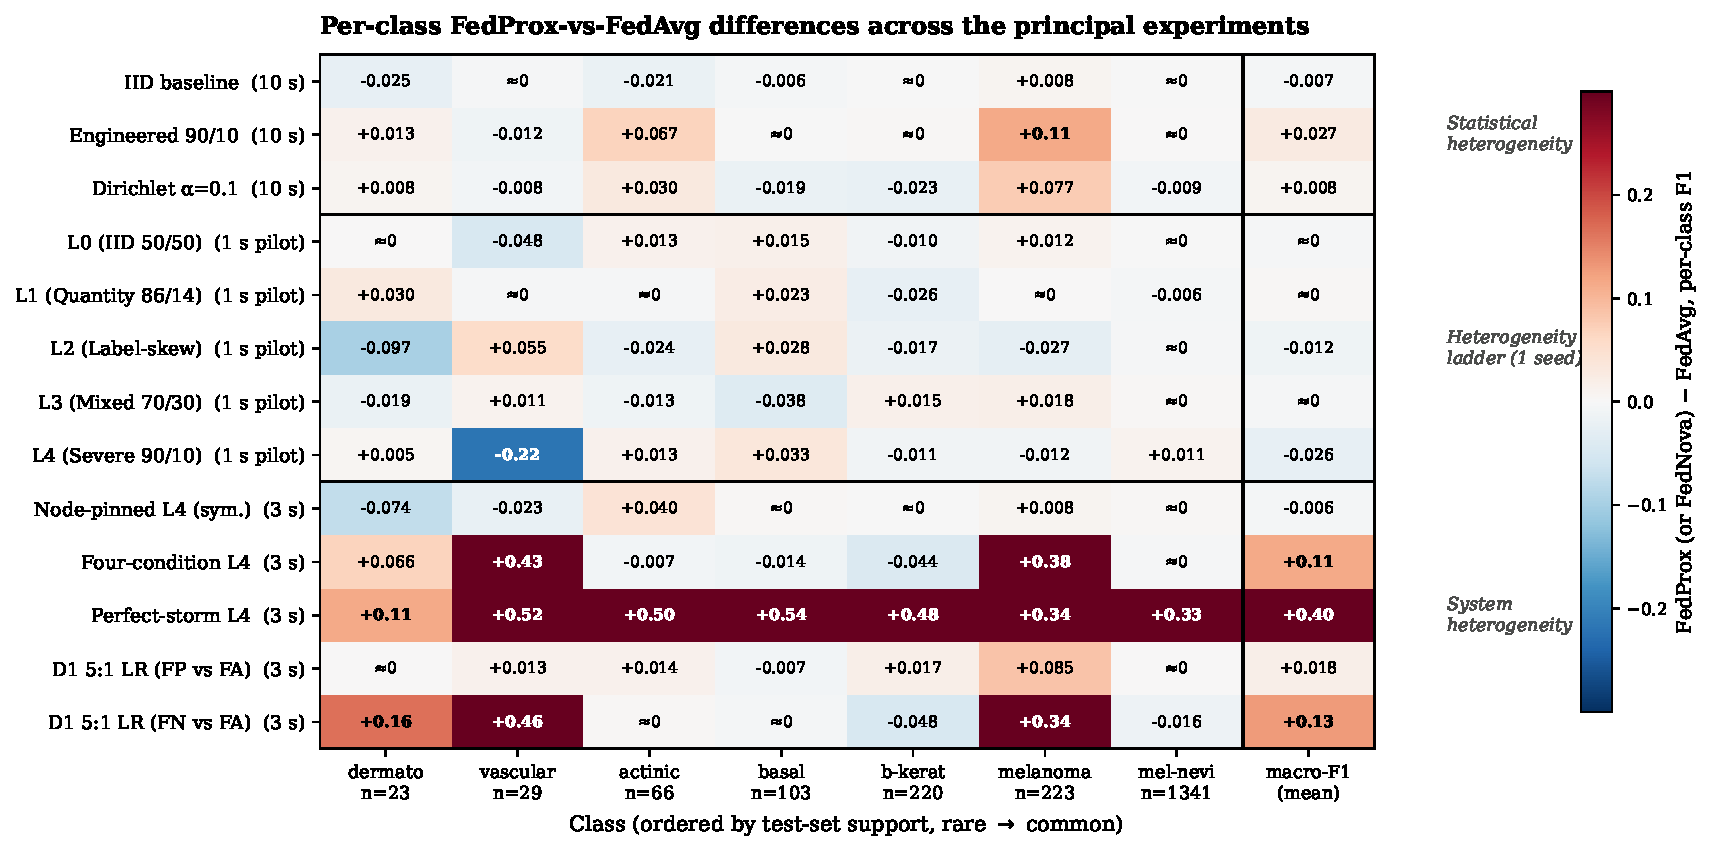
\includegraphics[width=\textwidth]{F_cross_experiment_per_class.pdf}
\caption{Per-class diagonal accuracy (correct-prediction rate per class)
across twelve protocol cells spanning baselines, Li 2020 straggler
conditions, perfect-storm, asymmetric LR (D1 1:1 and 5:1), and node-pinned
L4. The mel-nevi column saturates near $0.85$--$0.95$ in nearly every cell
while the dermato, melanoma, and vascular columns collapse to near zero in
the failing cells.}
\label{fig:cross-experiment-per-class}
\end{figure}



%%%%%%%%%%%%%%%%%%%%%%%%%%%%%%%%%%%%%%%%%%%%%%%%%%%%%%%%%%%%%%%%%%%%%%%%%%%%%%%
%% sec 5.7 -- Mechanism and robustness checks
%%%%%%%%%%%%%%%%%%%%%%%%%%%%%%%%%%%%%%%%%%%%%%%%%%%%%%%%%%%%%%%%%%%%%%%%%%%%%%%

% =============================================================================
% Results sec 5.7 -- Mechanism and robustness checks
% Compressed version. Target ~390 words.
% =============================================================================

\section{Mechanism and robustness checks}
\label{sec:mechanism-robustness}

\subsection*{\S\,5.7.1 Update-norm activity}

The update-norm logs are used here as a diagnostic: they measure how far a
client's local model moves away from the round-start global model. In other
words, $\lVert \Delta w \rVert$ is the size of the client update sent back to
the server. This helps separate two ideas that are easy to confuse. FedProx's
proximal term acts during local training and should make client updates
smaller. The $\gamma$-inexact policy acts later, at aggregation, by deciding
whether a straggler's partial update is accepted or dropped.

On the engineered partition ($n=10$), FedProx does reduce update size. The
mean per-round update norm is $1.523$ for FedAvg and $1.029$ for FedProx
($\mu=0.01$), a reduction of about $32\%$
(Figure~\ref{fig:update-norms}, trajectory panel). This confirms that the
FedProx proximal term is doing its intended local job: it keeps client models
closer to the global model. This does not contradict
Section~\ref{sec:li-straggler}.
There, the large straggler-regime gain came mainly from accepting the rare
client's partial update, not from the proximal term alone.

We then asked whether update size helps explain rare-class performance across
the L4 experiments. Across 78 L4 runs pooled from the baseline, Li-style
four-condition, perfect-storm, asymmetric-$\mu$, asymmetric-LR, and
weighted-CE experiments, larger Client 0 update norms tend to appear in runs
with higher rare-class F1 (Spearman $r=+0.634$;
Figure~\ref{fig:update-norms}, scatter panel). This should be read only as a
training-health signal: runs with healthier optimisation tend to have both
larger useful updates and better rare-class performance.

The rare client's update size is more informative only when the comparison is
made inside a single controlled protocol. Across all pooled L4 protocols, the
simple ratio between Client 1's update size and Client 0's update size is not
predictive of rare-class F1 (Spearman $r=-0.045$). This is because the pooled
runs mix different mechanisms: some drop stragglers, some accept partial
updates, some change the learning rate, some change $\mu$, and some change
the loss. The same update-size ratio can therefore mean different things in
different protocols.

Inside the asymmetric-LR experiment alone, the interpretation is cleaner
because the main change is Client 1's learning rate. In that setting, rare-class
F1 closely follows how strong Client 1's update remains relative to Client 0's:
$r=+0.80$ for FedAvg and $r=+0.87$ for FedProx
(cf.\ \S\,\ref{sec:lr-asymmetry}). This supports the interpretation from
\S\,\ref{sec:lr-asymmetry}: when the rare client's update becomes too small,
FedAvg and FedProx lose rare-class performance.

These update-norm results are therefore supporting evidence, not causal proof.
They show that FedProx reduces local update size, as expected, and that rare-
class performance can track the rare client's update strength inside a clean
learning-rate asymmetry experiment. The main mechanism claims still rest on
the controlled contrasts in \S\,\ref{sec:li-straggler} and
\S\,\ref{sec:lr-asymmetry}.
\subsection*{\S\,5.7.2 Protocol-flip audit}

The protocol-flip audit checks whether the reported algorithm ranking depends
on how performance is measured. For each selected L4 comparison, I compared
three reporting choices: the best-validation checkpoint, the final round, and
the mean over the last (K) rounds. A flip occurs when the sign of the paired
difference changes across these choices; for example, if FedProx is ahead at
the best-validation checkpoint but FedAvg is ahead at the final round.

The audit separates large effects from small effects. In the large-effect
settings, including the Li-style straggler decomposition and perfect-storm
experiments, none of the nine seed-level comparisons changed sign
((0/9) flips). In the small-effect settings, three of nine comparisons did
change sign ((3/9) flips). This means that sub-(1) percentage-point
differences are sensitive to the reporting protocol, while the large
asymmetric-protocol effects are not.

This affects how the chapter weights its conclusions. The centrepiece
\S\,\ref{sec:li-straggler} effect ($+0.115$ macro-F1) and the
\S\,\ref{sec:lr-asymmetry} FedNova--FedAvg gap at 50:1 ($+0.131$ macro-F1)
are large enough to survive checkpoint-choice changes. By contrast, the
small differences in \S\,\ref{sec:statistical-heterogeneity} should be
read as weak and fragile rather than as stable optimiser rankings.
\S\,5.8 therefore labels each finding by its strength.

Several additional diagnostics are kept in Appendix~E: the
(B)-dissimilarity proxy, the training-instability metric, the asymmetric
(\mu) Yao test, the early-warning collapse detector, and the small-hospital
case study. These checks are useful for interpretation, but none is used as
load-bearing evidence for the main conclusions in \S\S\,5.2--5.8.

Together, the update-norm and protocol-flip checks support the main message:
large regime-dependent effects are robust, while small symmetric-protocol
differences should be treated cautiously. The next section summarises this
regime map.
=============================================================================
% Figure 5.8 -- update-norm mechanism
% =============================================================================

\begin{figure}[H]
\centering
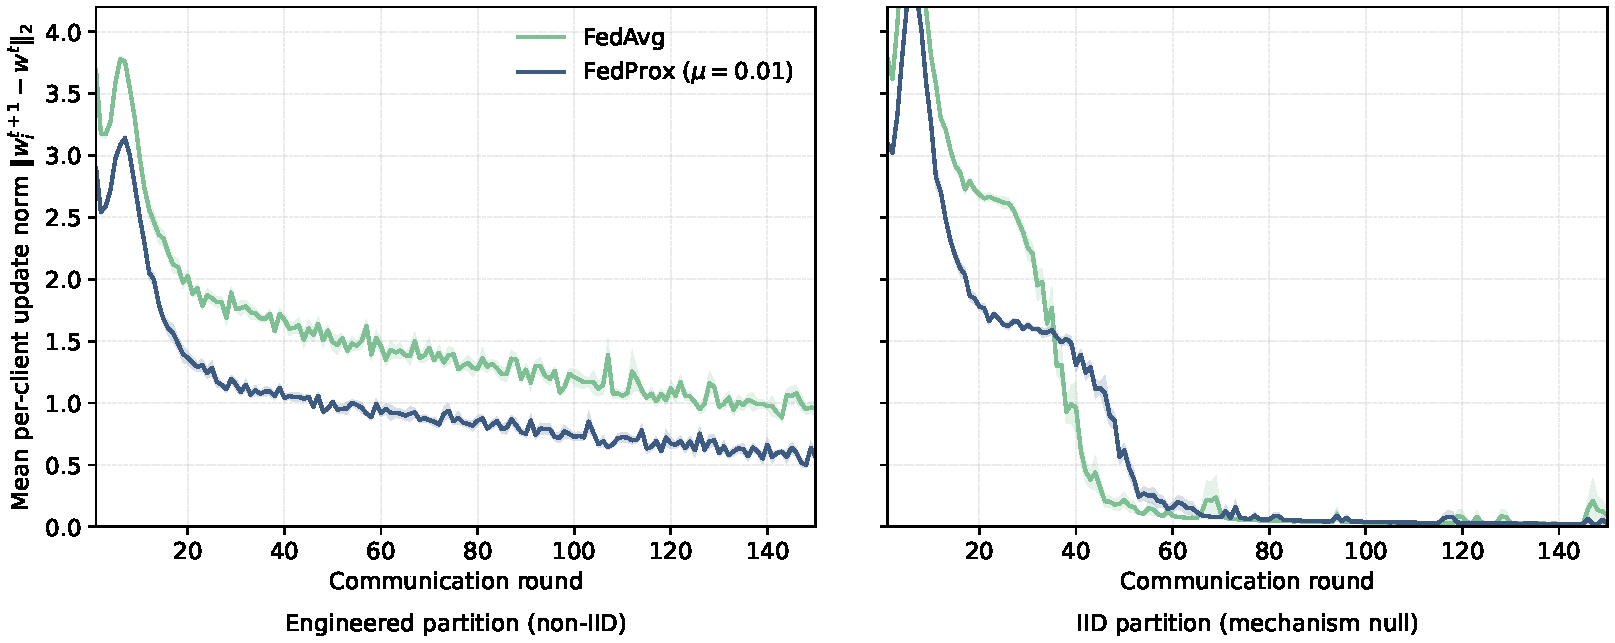
\includegraphics[width=0.85\textwidth]{F_update_norms.pdf}
\caption{Update-norm mechanism on the engineered partition. Mean per-round
$\lVert \Delta w \rVert$ trajectories per client for FedAvg vs FedProx
($n=10$ seeds); FedProx tracks lower throughout, consistent with the
proximal term's drift-control intent. Cross-protocol scatter panel
(78 L4 runs across 8 algorithm $\times$ protocol cells): Spearman
$r = +0.634$ between dominant-client mean update-norm and rare-class F1;
relative-influence ratio $r = -0.045$ across protocols.}
\label{fig:update-norms}
\end{figure}



%%%%%%%%%%%%%%%%%%%%%%%%%%%%%%%%%%%%%%%%%%%%%%%%%%%%%%%%%%%%%%%%%%%%%%%%%%%%%%%
%% sec 5.8 -- Integrated summary of findings
%%%%%%%%%%%%%%%%%%%%%%%%%%%%%%%%%%%%%%%%%%%%%%%%%%%%%%%%%%%%%%%%%%%%%%%%%%%%%%%

% =============================================================================
% Results sec 5.8 -- Integrated summary of findings
% Compressed. Target ~350 words. Closes with the central thesis sentence
% verbatim per guide sec 1.
% =============================================================================

\section{Integrated summary of findings}
\label{sec:integrated-summary}

Across the six experiments above, rare-class outcomes track rare-client
signal flow into the global model. FedAvg under stragglers drops the
rare-client update outright; FedProx with the proximal term alone does
not change which clients aggregate, so it cannot recover signal that was
discarded; FedProx + $\gamma$-inexact accepts partial rare-client updates
and recovers the signal; FedNova's $\tau$-normalisation rescales by
effective work and recovers signal under persistent LR asymmetry but
amplifies noise under random-$\tau$; weighted CE re-weights rare classes
during local training but only on clients that are actually aggregated.
The conditional thesis collapses to one rule: in these experiments,
optimiser/protocol cells preserve rare-class F1 when rare-client signal
continues to reach the global model. Table~\ref{tab:final-claims} reports the chapter's findings
with explicit strength labels; five take-aways anchor the regime map.

(1) Statistical heterogeneity alone yields a small, runtime-sensitive
FedProx--FedAvg separation: Flower paired $\Delta = +0.007$ on the
engineered partition ($n=10$, 7/10 paired wins) with the pure-PyTorch
$\Delta = +0.027$ as the upper end of a $0.01$--$0.03$ band; the IID
negative control is $\Delta = -0.007$.

(2) The proximal coefficient is sharply tuned: the $\mu$-sweep traces an
inverted-$U$ with a useful single-decade range around $\mu = 0.01$ and a
catastrophic $\Delta = -0.074$ at $\mu = 1.0$ ($n=10$, 0/10 paired wins).

(3) Under Li-style straggler asymmetry at L4, the total FedProx--FedAvg gap
is $+0.115$ ($n=3$), but only $+0.004$ comes from the proximal term ---
about $96\,\%$ of the gain is mediated by $\gamma$-inexact partial-update
handling. The L1 cross-partition control flattens the $\gamma$-inexact
contribution to $+0.012$, confirming that the mechanism operates only when
the dropped client carries informationally unique class signal.

(4) FedNova is regime-dependent in both directions: the 50:1 FedNova--FedAvg
gap is $+0.131$ macro-F1 (the largest single-axis system-asymmetry gap in
the thesis, $n=3$), while random-$\tau$ straggler heterogeneity collapses
FedNova to mean macro-F1 $= 0.237$ with three of ten seeds reduced to the
majority-class-only baseline.

(5) Across failing protocols, the clinically motivated failure mode is
rare-class collapse into mel-nevi ($24\,\%$ to $67\,\%$ misrouting), and
weighted CE on FedAvg ($0.505$, $n=3$) matches or exceeds FedProx+CE
($0.478$, $n=3$) in the tested L4 symmetric setting --- FedProx is best
understood as a drift/protocol intervention rather than a class-imbalance
corrector.

Federated optimiser performance in imbalanced medical FL is regime-dependent:
FedAvg remains competitive under IID or symmetric low-risk protocols;
FedProx becomes valuable under Li-style straggler asymmetry mainly because
$\gamma$-inexact partial-update handling preserves the rare-client signal;
FedNova is robust under the tested learning-rate asymmetry but fails under
random-$\tau$ straggler regimes; and across failing settings, the common
clinical failure mode is rare-class collapse into the majority class
(mel-nevi). These results do not establish a universal ranking of FedAvg,
FedProx, and FedNova. They instead map which optimiser/protocol choices
preserve or lose rare-class performance under different heterogeneity
regimes.


% =============================================================================
% Table 5.5 -- Final claim-evidence-caveat summary
% =============================================================================

\begin{table}[H]
\centering
\small
\caption{Final claim--evidence--caveat summary. Strength labels: \emph{strong}
= multi-seed, mechanism-isolable, checkpoint-robust; \emph{medium} =
multi-seed but small effect or single-protocol; \emph{exploratory} =
correlational, single-protocol, or $n=3$ without mechanism isolation.}
\label{tab:final-claims}
\begin{tabular}{p{3.0cm}p{3.6cm}p{1.6cm}p{2.6cm}p{2.6cm}}
\hline
Claim & Evidence & Strength & Caveat & Implication \\
\hline
FedProx not free under IID & Flower IID $\Delta = -0.007$ ($n=10$) & strong & IID is artificial & Reach for FedProx only when heterogeneity exists \\
Stat-het alone gives fragile separation & Flower engineered $\Delta = +0.007$ (7/10 wins, $n=10$) & medium & Runtime-sensitive (PyTorch $+0.027$) & Do not recommend FedProx on partition alone \\
$\mu$ must be tuned & Sweep $n=10$: peak $+0.013$ at $\mu = 0.01$; $-0.074$ at $\mu = 1.0$ & strong & Engineered partition only & Default $\mu = 0.01$; do not raise under heterogeneity \\
$\gamma$-inexact dominates straggler gain & L4 four-condition $n=3$: total $+0.115$, $\gamma$-inex $+0.111$; L1 control $+0.012$ & medium--strong & Simulated stragglers; no FedAvg+$\gamma$-inex standalone cell & Use FedProx + $\gamma$-inexact under straggler protocols \\
FedNova regime-dependent & LR envelope: FN holds $0.49$--$0.53$ across 1:1--50:1 ($n=3$); random-$\tau$ collapses to $0.237$ ($n=10$, 3/10 majority) & medium--strong & Wang 2020 stable-$\tau$ assumption violated by random-$\tau$ & Prefer FedNova under persistent LR asymmetry, not under random-$\tau$ \\
Rare-class collapse is the clinical failure mode & Misrouting $24\,\%$--$67\,\%$; D1 5:1 melanoma F1 $= 1.2$/$6.1$/$46.3\,\%$ ($n=3$) & strong & Single dataset, $28 \times 28$ resolution & Report per-class metrics; macro-F1 alone hides it \\
wCE competes with FedProx & L4 $n=3$: FA+wCE $0.505$ vs FP+CE $0.478$ & medium & $n=3$, L4 symmetric only & Loss-side rebalancing is a competitive intervention \\
Update-norms support drift-control reading & Engineered: FA $1.523$ vs FP $1.029$ ($-32\,\%$); cross-protocol $r = +0.634$ & exploratory & Within-protocol $r$ does not extrapolate & Drift-control reading is supported, not proven \\
\hline
\end{tabular}
\end{table}



%%%%%%%%%%%%%%%%%%%%%%%%%%%%%%%%%%%%%%%%%%%%%%%%%%%%%%%%%%%%%%%%%%%%%%%%%%%%%%%
%% sec 5.9 -- Limitations
%%%%%%%%%%%%%%%%%%%%%%%%%%%%%%%%%%%%%%%%%%%%%%%%%%%%%%%%%%%%%%%%%%%%%%%%%%%%%%%

% =============================================================================
% Results sec 5.9 -- Limitations
% Compressed. Target ~200 words. One-line bullets, terse.
% =============================================================================

\section{Limitations}
\label{sec:limitations}

\begin{itemize}
\setlength\itemsep{0.15em}
\item Single dataset at low resolution (DermaMNIST $28 \times 28$); no
replication on Camelyon, full-resolution ISIC, or non-dermatology MedMNIST
subsets.
\item Mixed federation sizes: 7-client for the engineered headline and
statistical-heterogeneity settings; 2-client for the mechanism probes
(Li 2020 four-condition, perfect-storm, asymmetric LR, weighted-CE,
asymmetric $\mu$, node-pinned L4). No cross-scale generalisation claim is
made between the two sizes.
\item Local-epoch budget fixed at $E = 20$; straggler protocols are
simulated via local-epoch counts rather than wall-clock deadlines.
\item $n = 3$ paired seeds for several strong asymmetry claims
(Li 2020 four-condition, perfect-storm, asymmetric LR, weighted-CE,
asymmetric $\mu$). No significance test is applied at this sample size.
\item The heterogeneity ladder is a single-seed pilot and is reported as
such; multi-seed promotion exists only at L4 ($n = 3$).
\item Runtime divergence between pure-PyTorch ($+0.027$) and Flower
($+0.007$) on the engineered partition limits magnitude claims; only
direction is robust across runtimes.
\item No SCAFFOLD, FedAdam, or FedYogi comparator; the optimiser space is
FedAvg, FedProx, FedNova only.
\item No AUC or calibration metrics; predictions are argmax only.
\item Per-client validation distributions were not logged centrally;
q-FFL-style fairness CDFs and Sheller-style cross-client generalisation
grids cannot be produced from existing artefacts.
\end{itemize}


%% =============================================================================
%% END OF RESULTS BODY
%% =============================================================================


%% =============================================================================
%% CHAPTER 6: DISCUSSION
%% =============================================================================
\chapter{Discussion}
\label{ch:discussion}

%% TODO: target 2,000-3,000 words.

\section{Re-stating the regime map}
\label{sec:disc-regime-map}
%% Recap the central conditional thesis from sec 5.8.

\section{Mechanism interpretation: signal flow as the unifying rule}
\label{sec:disc-signal-flow}
%% The sec 5.8 unifying observation: rare-class F1 is preserved iff rare-
%% client signal reaches the global model. Discuss why this collapses six
%% experiments into one rule.

\section{Implications for cross-hospital federated medical learning}
\label{sec:disc-implications}
%% What does the regime map suggest for actual hospital FL deployments?
%% Distinguish recommendations by the kind of heterogeneity expected.

\section{Comparison with prior work}
\label{sec:disc-prior-work}
%% Where this thesis confirms, extends, or contradicts Li 2020, Wang 2020,
%% McMahan 2017. Hedge appropriately --- per guide sec 8 do not say "this
%% refutes ...".

\section{Threats to validity}
\label{sec:disc-validity}
%% Internal: n=3, simulated stragglers, runtime divergence.
%% External: single dataset, low resolution, mixed federation sizes.
%% Construct: rare-class definition includes melanoma (mid-support, high-stakes).


%% =============================================================================
%% CHAPTER 7: CONCLUSION
%% =============================================================================
\chapter{Conclusion}
\label{ch:conclusion}

%% TODO: target 500-800 words.

\section{Summary of contributions}
\label{sec:conc-summary}
%% Re-state the four or five main contributions from sec~1.3.

\section{Practical recommendations}
\label{sec:conc-recommendations}
%% One-paragraph recommendation per regime cell. E.g.,
%%   - "Under IID-like client distributions, no FL optimiser dominates."
%%   - "Under straggler protocols on heterogeneous data, prefer FedProx + gamma-inexact."
%%   - "Under persistent LR asymmetry, prefer FedNova; under random-tau, prefer FedAvg/FedProx."
%%   - "Loss-side rebalancing (weighted CE) is a competitive complement, not a substitute."

\section{Future work}
\label{sec:conc-future-work}
%% Items naturally extending the thesis:
%%   - SCAFFOLD/FedAdam/FedYogi comparators
%%   - Cross-dataset validation (Camelyon, full-resolution ISIC)
%%   - Real wall-clock straggler protocols
%%   - Per-client validation logging for fairness CDFs
%%   - Combining gamma-inex aggregation with weighted-CE local objective


%% =============================================================================
%% BIBLIOGRAPHY
%% =============================================================================
\bibliographystyle{plainnat}
\bibliography{references}


%% =============================================================================
%% APPENDICES  (per THESIS_BUILD_GUIDE.md sec 7)
%% =============================================================================
\appendix

\chapter{Supplementary statistical heterogeneity}
\label{app:stat-het}
%% Full heterogeneity ladder; full Dirichlet seed table; specialist details;
%% pure-PyTorch vs Flower equivalence notes.

\chapter{$\mu$ and FedProx sensitivity}
\label{app:mu-sensitivity}
%% mu x ladder cross-partition pilot (mu_sweep_ladder/);
%% per-class mu at L0/L2 if not in main;
%% extended-rounds L3 (250 rounds);
%% asymmetric mu Yao test.

\chapter{System heterogeneity and FedNova diagnostics}
\label{app:system-het}
%% Perfect-storm convergence figure (panel B);
%% FedNova random-tau trajectories;
%% FedNova unequal-E pilot;
%% partial participation C=0.5.

\chapter{Rare-class and clinical failure diagnostics}
\label{app:clinical}
%% D1 5:1 confusion matrices;
%% collapse trajectory plots;
%% small-hospital case study;
%% early-warning collapse detector (labelled exploratory).

\chapter{Robustness and mechanism audits}
\label{app:robustness}
%% Protocol-flip detailed table;
%% B-dissimilarity proxy;
%% training-instability metric;
%% cross-protocol mechanism scatter if not in main;
%% arch_ablation_bn one-paragraph BatchNorm note.

\end{document}
